% === 数值口径（来源：artifacts/q1/data/strategy_comparison.csv, questions/q1/artifacts/tables/validation_summary.csv, questions/q1/artifacts/tables/sensitivity_summary.csv, 2026-07-06） ===
% Q1: 等速策略 final_time=761.917s, final_distance=200668.442m, final_height=10637.065m, fuel=10450.000kg, mean_climb=1.492374m/s, max_climb=1.492374m/s
% Q1: 等马赫策略 final_time=811.032s, final_distance=211331.296m, final_height=10437.818m, fuel=10450.000kg, mean_climb=1.156327m/s, max_climb=1.204912m/s
% Q1: CL_ref=0.658914, sqrt(CD0/k)=0.699206
% Q1: cT主=2.8e-4, 对照=2.8e-5
% Q1: beta扰动[-20%,-10%,+10%,+20%]
% Q1: 风场 W(h)=20+3e-5*(h-10000)^2

% \documentclass{cumcmthesis}
\documentclass[withoutpreface,bwprint]{cumcmthesis}
\usepackage{seqsplit}
% === cumcmthesis 元信息 ===
\title{基于点质量模型的民用客机巡航爬升轨迹与燃油优化}
\tihao{A}
\baominghao{}
\schoolname{}
\membera{ }
\memberb{ }
\memberc{ }
\supervisor{ }
\yearinput{2026}
\monthinput{7}
\dayinput{6}

% === cumcmthesis 未加载的宏包 ===
\usepackage{algorithm}
\usepackage{algpseudocode}
\usepackage{hyperref}
\usepackage{cite}
\usepackage{fancyhdr}
\usepackage{setspace}
\usepackage{enumitem}
\usepackage{float}

% === 页面设置 ===
\pagestyle{fancy}\fancyhf{}\cfoot{\thepage}
\renewcommand{\headrulewidth}{0pt}
\fancypagestyle{plain}{\fancyhf{}\renewcommand{\headrulewidth}{0pt}\cfoot{\thepage}}

% === 行距设置（统一 1.25）===
\setstretch{1.25}

% === 标题编号：一级用汉字（一、二、三），二三级用阿拉伯数字（1.1、1.1.1） ===
\renewcommand{\thesection}{\chinese{section}、}
\renewcommand{\thesubsection}{\arabic{section}.\arabic{subsection}}
\renewcommand{\thesubsubsection}{\arabic{section}.\arabic{subsection}.\arabic{subsubsection}}

% === 代码高亮设置（覆盖 cumcmthesis 默认设置） ===
\lstset{
  basicstyle=\zihao{5}\ttfamily,
  numbers=left,
  numberstyle=\tiny,
  breaklines=true,
  frame=single,
  keepspaces=true,
  columns=flexible
}

\hypersetup{colorlinks=true,linkcolor=black,citecolor=black,urlcolor=blue,bookmarks=true}
\graphicspath{{figures/}{questions/q1/artifacts/figures/}{questions/q2/artifacts/figures/}{../artifacts/q1/data/}{artifacts/q1/data/}}

\begin{document}

% === 行距设置（统一 1.25）===
\setstretch{1.25}

\maketitle

\begin{abstract}\setstretch{1.13}
针对民用客机巡航阶段燃油消耗集中、飞行高度与速度相互制约且高空风场不可忽略的特点，本文围绕高度、速度、质量、阻力、油耗和风场之间的耦合关系，建立"经验策略基线--固定路径油耗积分--无风最优控制--有风综合比较"的递进模型框架。模型以点质量动力学、升阻平衡和燃油率方程为基础，并在不同子问题中分别固定终止质量、共同航程或终端机械状态，使策略比较、油耗复算和优化建模具有一致的物理口径。

\textbf{对于问题一，}建立小航迹角准稳态点质量模型，将水平运动、质量衰减、升力平衡、阻力计算和燃油率方程统一到时间域中，并以参考升力系数作为闭合条件描述等速和等马赫两类经验巡航爬升策略。在终止质量 $62000\ \mathrm{kg}$ 下，两策略总油耗均为 $10450\ \mathrm{kg}$；等速策略最终高度 $10637.065\ \mathrm{m}$、时间 $761.917\ \mathrm{s}$，等马赫策略最终高度 $10437.818\ \mathrm{m}$、时间 $811.032\ \mathrm{s}$、航程 $211331.296\ \mathrm{m}$。结果表明，固定终止质量口径下油耗不再区分策略，比较重点应转向高度剖面、时间剖面和航程差异；等马赫策略航程增大主要来自飞行时间延长，而终点高度较低由声速随高度下降和升力平衡共同造成。

\textbf{对于问题二，}在问题一等速几何路径上建立燃油路径积分模型，把标准 ISA 中温度、压力、密度和声速的高度连续分布传递到升力系数、阻力、推力需求和燃油率计算中。为避免固定终止质量掩盖大气修正的影响，本文采用共同可行航程 $189781.310\ \mathrm{m}$ 作为比较基准；标准 ISA 总油耗为 $10427.256\ \mathrm{kg}$，$+10\ \mathrm{K}$ 静力温差修正后为 $10450.000\ \mathrm{kg}$，增加 $22.744\ \mathrm{kg}$，相对增加 $0.218\%$。时间域和路径域复算保持一致，静力平衡残差约为 $10^{-10}$ 量级，说明积分口径和非标准大气处理均较稳定；$|\Delta T|\leq10\ \mathrm{K}$ 时油耗变化小于 $0.3\%$，在当前参数和航程尺度下可把常温偏差视为二阶修正。

\textbf{对于问题三，}将经验策略推广为固定航程、固定终端高度和速度、终端质量自由的最优控制问题，以最大化终端质量等价刻画最小油耗，避免"固定终止质量再最小化油耗"的目标退化。先用航程域直接配点构造连续可行初值，再以 reduced-control shooting 进行最终燃油优化。无风优化在 $241$ 节点网格上得到总油耗 $10342.814\ \mathrm{kg}$、终端质量 $62107.186\ \mathrm{kg}$、终端时间 $805.679\ \mathrm{s}$，相对可行初值 $10450.000\ \mathrm{kg}$ 降低约 $107.186\ \mathrm{kg}$。连续验证表明终端速度重积分误差 $1.71\times10^{-5}\ \mathrm{m/s}$、燃油恒等式残差 $8.58\times10^{-5}\ \mathrm{kg}$，无风最终燃油优化已形成可复核结果。

\textbf{对于问题四，}在问题三无风最优基础上引入有风航程域最优控制，采用 reduced-control shooting 局部优化。固定共同航程 $189781.310\ \mathrm{m}$ 下，有风局部优化轨迹总油耗 $9863.840\ \mathrm{kg}$，比等速基线节省 $563.416\ \mathrm{kg}$（$5.403\%$）；固定燃油 $10450\ \mathrm{kg}$ 口径下可达航程下界估计 $201168.189\ \mathrm{m}$，较共同航程增加 $11386.879\ \mathrm{m}$。速度偏离惩罚系数 $\beta$ 从标称值降至 $0.8$ 倍时局部可行解燃油减少 $14.116\ \mathrm{kg}$，增至 $1.2$ 倍时增加 $6.230\ \mathrm{kg}$。

本文形成的"经验策略基线--路径油耗积分--无风最优控制--有风综合比较"四层递进框架表明，不同子问题必须匹配不同评价口径，固定终止质量、固定航程和固定终端机械状态各有适用场景。

\keywords{巡航爬升；燃油路径积分；静力温差修正；直接配点；最优控制}
\end{abstract}

\section{问题重述}

\subsection{问题背景}

巡航阶段是民用客机燃油消耗最集中的飞行阶段之一，也是航空公司降低运营成本和排放强度的重要环节。巡航爬升过程中，飞行高度改变大气密度和声速，飞行速度影响升阻特性与空中时间，燃油消耗引起飞机质量持续下降，高空风场又改变空速到地速的转换关系。上述因素共同决定单位航程油耗，因此本题的核心不是单独优化高度或速度，而是在给定飞机与大气条件下刻画二者的联合变化规律。

题目给出某型客机的质量、机翼面积、阻力极曲线、发动机油耗参数、标准大气近似和高度相关风场等参数，并指定初始高度 $9500\ \mathrm{m}$、初始空速 $240\ \mathrm{m/s}$ 与终止剩余质量 $62000\ \mathrm{kg}$。据此需建立可用于轨迹计算、油耗积分和策略比较的巡航模型，为传统经验策略与优化策略的定量评价提供统一基础。

\begin{figure}[H]
\centering
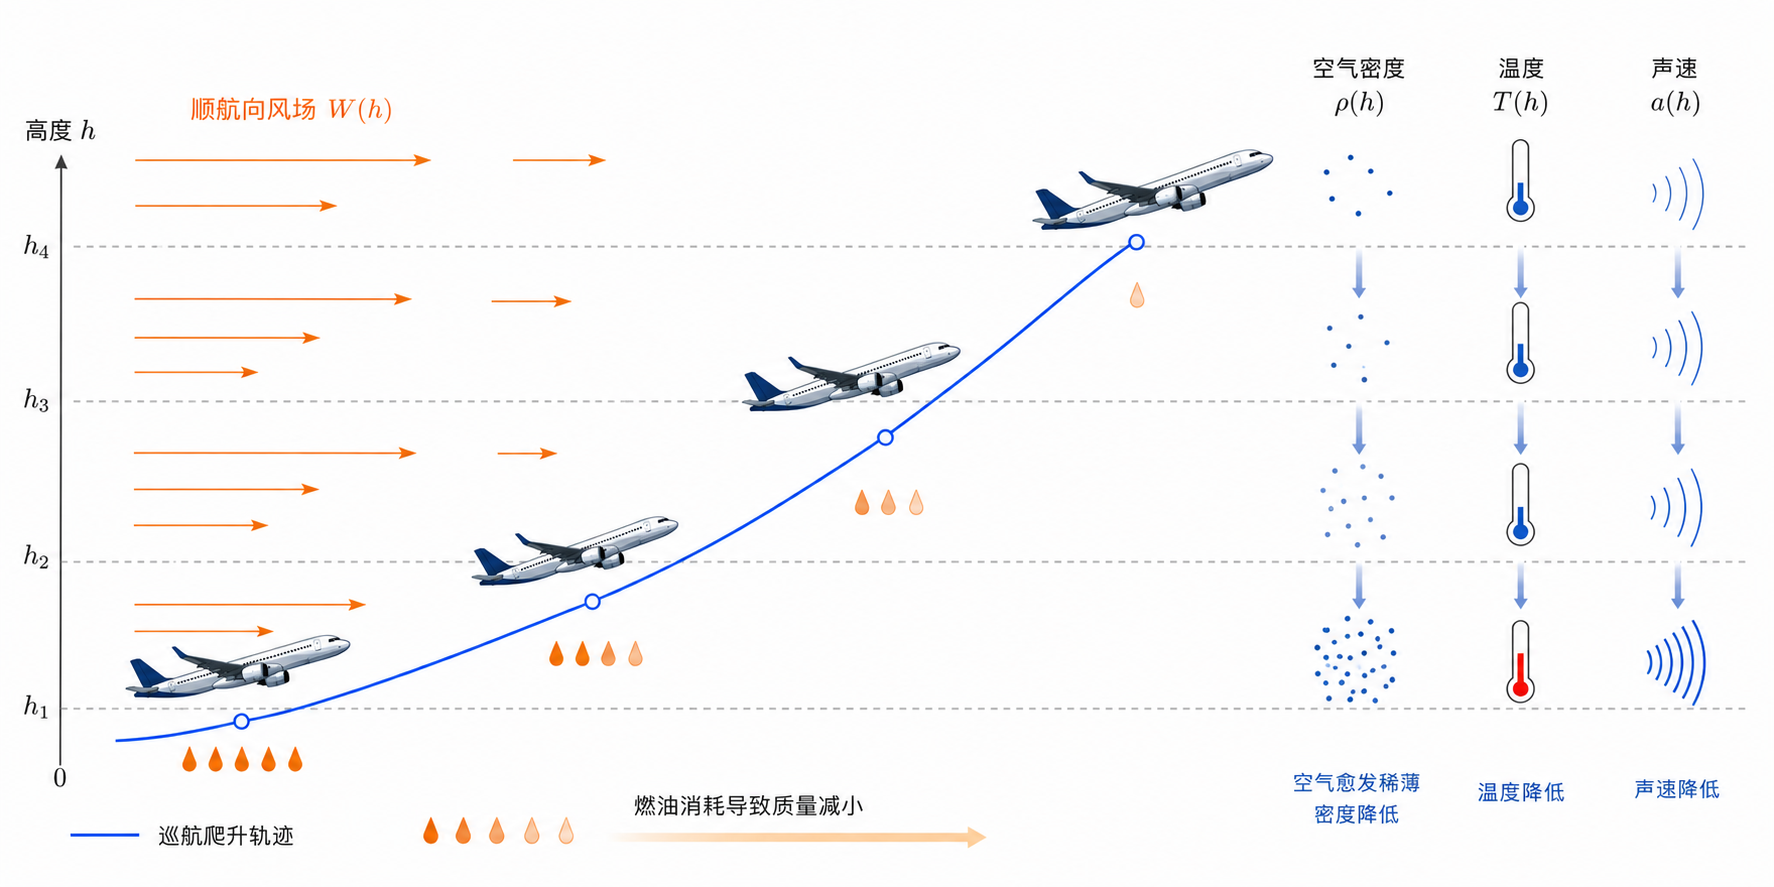
\includegraphics[width=0.9\textwidth]{fig_background_scene.png}
\caption{民用客机巡航爬升物理场景示意图}
\label{fig:background}
\end{figure}

\subsection{问题提出}

围绕该型客机巡航过程中的高度--速度联合决策，现要求我们解决以下问题：

\textbf{问题一：}在给定飞机气动和油耗参数下，建立描述高度、速度、航程和质量随时间变化的巡航动力学模型；以等速和等马赫数两类经验策略为对象，计算其高度、质量、飞行时间和燃油消耗，并比较两种策略的爬升特征。

\textbf{问题二：}将问题一得到的飞行过程转化为沿航程的燃油积分问题，重点考察大气温度、密度和声速随高度变化对油耗率的影响；在标准大气和温度偏差条件下分别计算总油耗，判断温度修正对最终结果的影响是否显著。

\textbf{问题三：}把高度和速度由预设经验策略推广为待优化轨迹，在动力学约束、飞行包线和终端要求下建立最小油耗模型；给出最优性条件和数值求解思路，并分析无风、有风及能量高度简化三种口径下模型结构的变化。

\textbf{问题四：}整合前三问模型形成综合计算框架，在问题三无风最优轨迹基础上引入有风航程域最优控制，对经验策略和有风优化策略进行同口径比较，输出燃油节省、航程变化和关键参数敏感性结论；同时给出若干面向工程应用的模型扩展方向。

\section{问题分析}

巡航爬升本质上是能量管理和气动约束共同作用下的轨迹优化问题。相关飞行动力学教材通常以点质量模型、升阻极曲线和飞行包线刻画巡航阶段的主要物理关系\cite{raymer,anderson,cook}；在数值求解层面，直接配点和 shooting 方法常用于把连续最优控制问题转化为带约束的非线性规划\cite{hargraves,betts}。因此，本文将四个问题组织为由经验策略到最优控制、由无风到有风的递进链条，并用独立重积分和灵敏度分析限定各结论的适用范围。

\subsection{问题一：经验策略闭合与动力学积分}

问题一的输入是初始状态、终止质量和两类经验速度策略，输出应包括高度、航程、时间和燃油消耗。其建模难点在于：等速或等马赫只限定速度变化，并不能单独决定巡航爬升高度。本文以小航迹角准稳态模型连接升力平衡、能量方程和质量衰减，再用参考升力系数保持不变补足高度闭合条件。这样，等速与等马赫策略可在同一气动假设下积分求解，比较结果也不依赖额外人为控制律。

\subsection{问题二：固定路径油耗与大气修正}

问题二继承问题一的等速几何路径，但评价对象从“达到给定终止质量”转为“同一航程下消耗多少燃油”。若继续固定终止质量，各大气场景总油耗都会等于 $m_0-m_f$，温差影响被比较口径抵消。本文固定路径和真空速，在标准 ISA 与常温偏差大气下重新计算密度、声速、升力系数、阻力和推力需求，并用共同可行航程统一比较区间。温差模型同步修正压力和密度，使静力平衡成立，从而把温度偏差的作用限定为同一几何路径上的气动与油耗变化。

\subsection{问题三：固定端点的高度--速度最优控制}

问题三把固定经验策略推广为高度--速度联合优化。此时决策变量不再是单一策略参数，而是整条轨迹上的高度、速度、推力和航迹角。若固定终止质量再最小化油耗，目标函数会退化；若终端高度和速度自由，又可能通过降低终端机械能得到虚假省油。因此本文固定航程、终端高度和终端速度，并以最大化终端质量表示最小油耗。考虑到模型含非线性阻力、质量变化和路径约束，数值上先采用航程域直接配点构造连续可行初值，再用 reduced-control shooting 求解无风最终燃油优化；PMP 必要条件用于解释最优性结构和后续诊断，不作为当前主要求解器。

\subsection{问题四：综合比较与灵敏度分析}

问题四以前三问的计算结果为基础，在问题三无风最优轨迹上引入有风航程域最优控制，定量比较等速经验策略与有风最优策略在固定共同航程下的燃油消耗差异。同时，在固定燃油预算口径下估计可达航程下界，并对速度偏离惩罚系数 $\beta$ 进行逐场景重新求解式灵敏度分析，讨论模型扩展方向。

\begin{figure}[H]
\centering
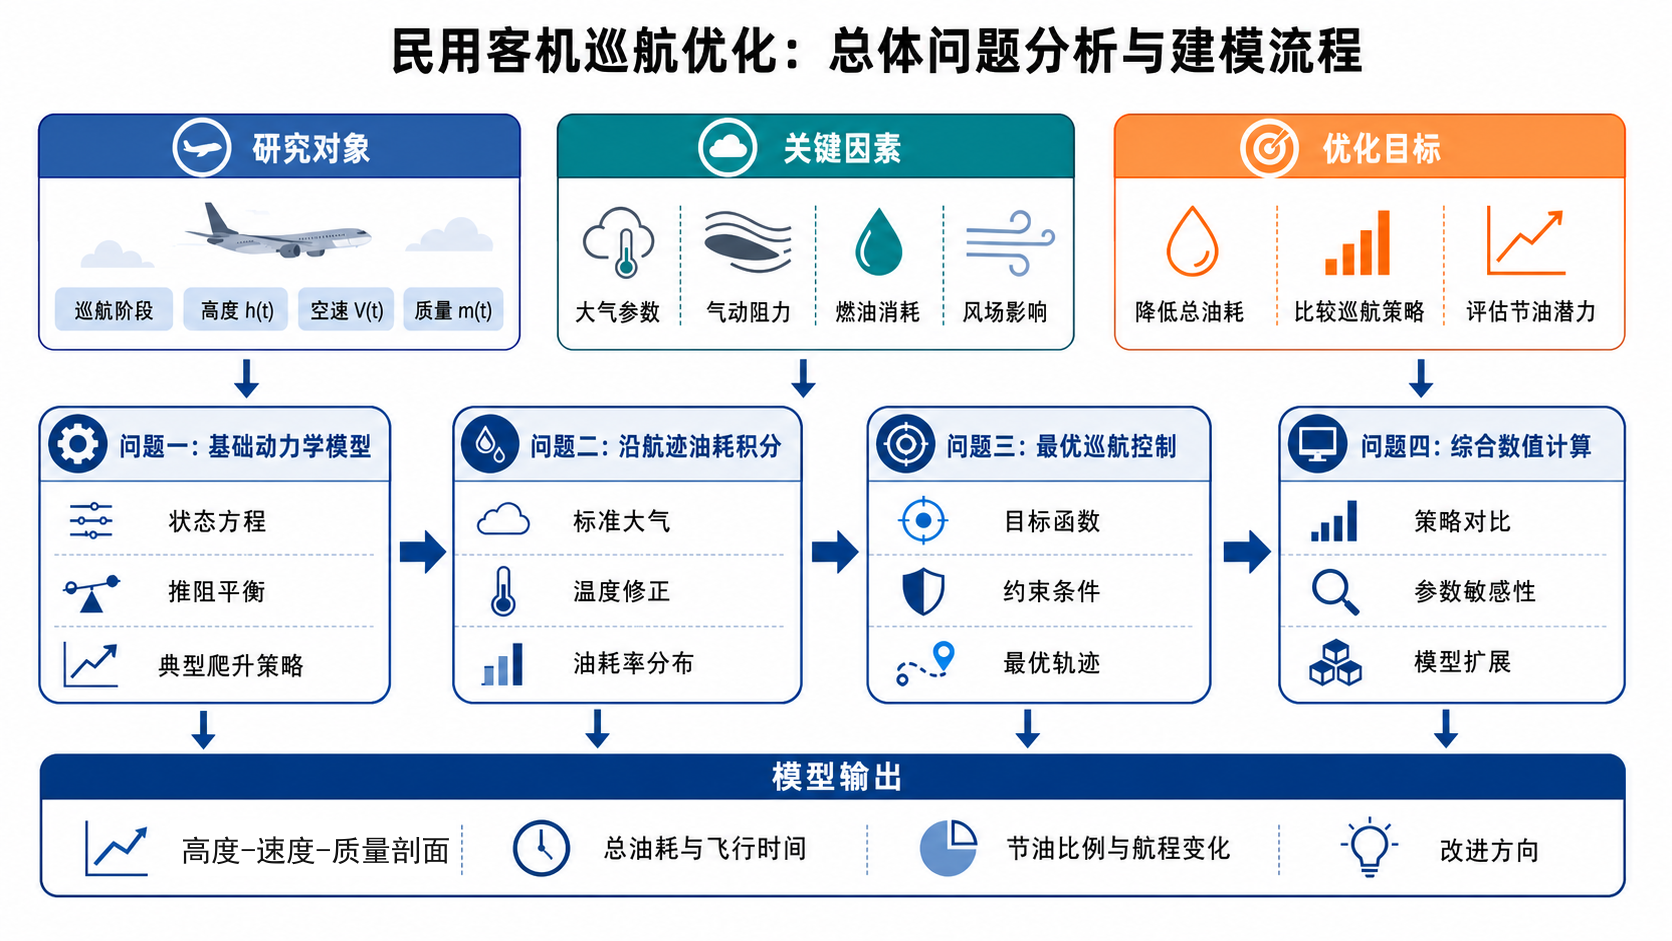
\includegraphics[width=0.9\textwidth]{overall_problem_analysis_modeling_flow.png}
\caption{总体问题分析与建模流程图}
\label{fig:modelflow}
\end{figure}

\section{模型假设}

\begin{enumerate}[left=0pt]
\item \textbf{小航迹角准稳态。}巡航爬升过程中航迹角较小，升力近似平衡重力，地速近似为空速与风速之和。
\item \textbf{参考升力系数闭合。}题目仅给出策略名称而未给推力包线，故采用参考升力系数保持不变的闭合条件使两类策略可比。
\item \textbf{风场仅随高度变化。}风速正值表示顺航向风，风场只随高度变化，不考虑时间和水平位置变化。
\item \textbf{抛物线阻力极曲线。}阻力系数由零升阻力系数与升致阻力因子的抛物线关系确定，不引入跨音速波阻项。
\item \textbf{题设燃油消耗系数。}主结果采用题设推力燃油消耗系数，另以低一个数量级的值作工程合理性对照，不静默替换题设值。
\end{enumerate}
\newpage
\section{符号说明}

\begin{table}[htpb]
\centering
\caption{本文的主要符号说明}\label{tab:symbols}
\begin{tabular}{cll}\toprule
符号 & 含义 & 单位 \\
\midrule
$t$ & 飞行时间 & s \\
$x(t)$ & 相对地面水平距离 & m \\
$h(t)$ & 飞行高度 & m \\
$V(t)$ & 真空速 & m/s \\
$m(t)$ & 飞机质量 & kg \\
$T(t)$ & 发动机推力 & N \\
$D(t)$ & 气动阻力 & N \\
$L(t)$ & 升力 & N \\
$S$ & 机翼面积 & $\mathrm{m^2}$ \\
$C_L$ & 升力系数 & -- \\
$C_D$ & 阻力系数 & -- \\
$C_{D0}$ & 零升阻力系数 & -- \\
$k$ & 升致阻力因子 & -- \\
$\rho(h)$ & 高度 $h$ 处空气密度 & $\mathrm{kg/m^3}$ \\
$a(h)$ & 高度 $h$ 处声速 & m/s \\
$M$ & 马赫数 & -- \\
$W(h)$ & 顺航向风速 & m/s \\
$c_T$ & 推力燃油消耗系数 & $\mathrm{kg/(N\cdot s)}$ \\
$\beta$ & 速度偏离惩罚系数 & $\mathrm{s^2/m^2}$ \\
$V_{\mathrm{opt}}$ & 最佳效率速度 & m/s \\
$m_0,m_f$ & 初始质量、终止质量 & kg \\
\bottomrule
\end{tabular}
\end{table}

\section{问题一模型的建立与求解}

\subsection{数据预处理}

计算前先统一题设参数和单位。飞机初始质量为 $m_0=72450\ \mathrm{kg}$，终止质量为 $m_f=62000\ \mathrm{kg}$，初始高度和真空速分别为 $h_0=9500\ \mathrm{m}$、$V_0=240\ \mathrm{m/s}$。气动参数取机翼面积 $S=112.3\ \mathrm{m^2}$、零升阻力系数 $C_{D0}=0.022$、升致阻力因子 $k=0.045$；燃油模型取推力燃油消耗系数 $c_T=2.8\times 10^{-4}\ \mathrm{kg/(N\cdot s)}$、速度偏离惩罚系数 $\beta=0.003\ \mathrm{s^2/m^2}$ 和最佳效率速度 $V_{\mathrm{opt}}=235\ \mathrm{m/s}$。

大气密度采用指数近似 $\rho(h)=\rho_0\exp(-h/H_\rho)$，其中 $\rho_0=1.225\ \mathrm{kg/m^3}$、$H_\rho=7300\ \mathrm{m}$；声速采用标准对流层近似 $a(h)=\sqrt{\gamma R T_{\mathrm{atm}}(h)}$，其中 $T_{\mathrm{atm}}(h)=T_0-L_T h$。风场按题设确认公式 $W(h)=20+3\times 10^{-5}(h-10000)^2\ \mathrm{m/s}$ 计算，正值表示顺航向风。上述预处理保证质量、长度、速度和油耗系数在后续方程中使用同一单位体系。

\subsection{模型建立}

小航迹角准稳态巡航爬升满足以下基本方程\cite{raymer,cook}。

水平地面距离变化由空速和风速共同决定：
\begin{equation}
\frac{dx}{dt}=V+W(h).
\label{eq:dxdt}
\end{equation}

升力近似平衡重力：
\begin{equation}
L=\frac{1}{2}\rho(h)V^2SC_L\approx mg,
\label{eq:lift}
\end{equation}
因此升力系数为
\begin{equation}
C_L=\frac{2mg}{\rho(h)V^2S}.
\label{eq:CL}
\end{equation}

阻力系数采用抛物线阻力极曲线\cite{anderson}：
\begin{equation}
C_D=C_{D0}+kC_L^2,
\label{eq:CD}
\end{equation}
阻力为
\begin{equation}
D=\frac{1}{2}\rho(h)V^2SC_D.
\label{eq:drag}
\end{equation}

小航迹角下，纵向能量方程可写为
\begin{equation}
m\frac{dV}{dt}=T-D-mg\sin\gamma\approx T-D-mg\frac{1}{V}\frac{dh}{dt},
\label{eq:energy}
\end{equation}
即
\begin{equation}
T=D+m\frac{dV}{dt}+\frac{mg}{V}\frac{dh}{dt}.
\label{eq:thrust}
\end{equation}

燃油消耗率采用题设的速度偏离惩罚形式：
\begin{equation}
\frac{dm}{dt}=-c_TT\left[1+\beta(V-V_{\mathrm{opt}})^2\right].
\label{eq:fuel}
\end{equation}
其中括号内为无量纲惩罚项，当 $V$ 偏离最佳效率速度 $V_{\mathrm{opt}}$ 时，单位推力燃油消耗率增加。

\eqref{eq:lift}--\eqref{eq:fuel} 构成巡航爬升的基本动力学模型。模型中，高度 $h(t)$ 和空速 $V(t)$ 决定气动状态与推力需求，水平距离 $x(t)$ 和飞机质量 $m(t)$ 则记录航程推进和燃油消耗；后续两类经验策略的差别体现在 $h(t)$ 与 $V(t)$ 的闭合方式上。

\subsection{闭合条件与两类巡航爬升策略}

题目要求比较等速巡航爬升与等马赫数巡航爬升，但这两种策略本身只约束速度或马赫数，尚不能唯一给出高度演化。为使两种策略在同一气动基准下比较，本文采用统一闭合条件
\begin{equation}
C_L=C_{L,\mathrm{ref}}=\frac{2m_0g}{\rho(h_0)V_0^2S}.
\label{eq:CL_ref}
\end{equation}
由题设初始状态计算得
\begin{equation}
C_{L,\mathrm{ref}}=0.658914.
\label{eq:CL_ref_val}
\end{equation}
该值接近抛物线阻力极曲线下最大升阻比升力系数
\begin{equation}
C_{L,(L/D)_{\max}}=\sqrt{\frac{C_{D0}}{k}}=0.699206.
\label{eq:CL_maxLD}
\end{equation}
因此，固定参考升力系数可解释为飞机通过迎角调整维持接近高升阻比的巡航爬升状态。该闭合条件不是唯一控制律，但能在题面未给推力包线和迎角控制细节时给出可复算的策略基线。下面分别写出等速和等马赫两种策略下的闭合关系，再用图形对两者的物理差异作直观说明。

\textbf{策略A：等真空速巡航爬升。} 令
\begin{equation}
V(t)=V_0=240\ \mathrm{m/s}.
\label{eq:const_V}
\end{equation}
由 $C_L=C_{L,\mathrm{ref}}$ 与升力平衡 \eqref{eq:lift} 可得
\begin{equation}
\frac{m(t)}{m_0}=\frac{\rho(h(t))}{\rho(h_0)}.
\label{eq:m_rho_ratio}
\end{equation}
代入指数密度模型 $\rho(h)=\rho_0\exp(-h/H_\rho)$，得到高度与质量关系：
\begin{equation}
h(t)=h_0-H_\rho \ln\frac{m(t)}{m_0}.
\label{eq:h_vs_m_constV}
\end{equation}
因此
\begin{equation}
\frac{dh}{dm}=-\frac{H_\rho}{m},\qquad \frac{dV}{dm}=0.
\label{eq:deriv_constV}
\end{equation}

\textbf{策略B：等马赫数巡航爬升。} 令
\begin{equation}
M(t)=M_0=\frac{V_0}{a(h_0)},\qquad V(t)=M_0a(h(t)).
\label{eq:const_M}
\end{equation}
由升力闭合条件 \eqref{eq:lift}--\eqref{eq:CL_ref} 可得
\begin{equation}
\frac{m(t)}{m_0}
=\frac{\rho(h(t))a^2(h(t))}{\rho(h_0)a^2(h_0)}.
\label{eq:m_rho_a2}
\end{equation}
对其求微分，得到
\begin{equation}
\frac{dh}{dm}
=\frac{1}{m\left[\dfrac{d\ln\rho}{dh}+2\dfrac{d\ln a}{dh}\right]},
\label{eq:dhdm_mach}
\end{equation}
并且
\begin{equation}
\frac{dV}{dm}=V\frac{d\ln a}{dh}\frac{dh}{dm}.
\label{eq:dVdm_mach}
\end{equation}

由上述两组关系可知，两种策略都由升力平衡闭合高度，但等速策略只通过密度降低来适应质量下降，等马赫策略还叠加了声速随高度下降引起的空速变化。图 \ref{fig:q1_closure} 将这种“同一质量衰减、不同高度闭合”的差异直接画出。

\begin{figure}[H]
\centering
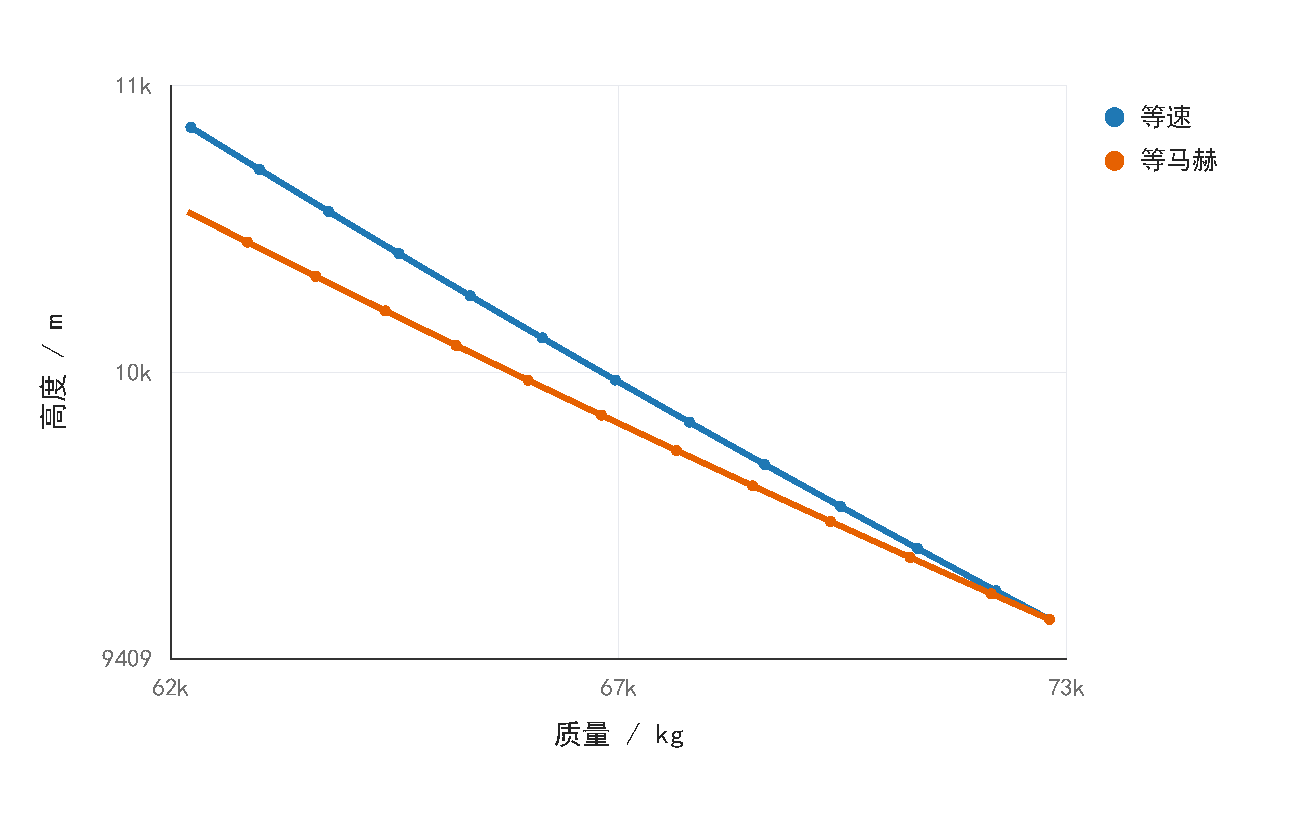
\includegraphics[width=0.86\textwidth]{fig_v2_q1_closure_mechanism.pdf}
\caption{问题一两类经验策略的升力平衡闭合机理}
\label{fig:q1_closure}
\end{figure}

由图 \ref{fig:q1_closure} 可见，质量从 $72450\ \mathrm{kg}$ 降至 $62000\ \mathrm{kg}$ 时，两类策略均随质量降低而爬升；等速策略马赫数随高度升高而增大，等马赫策略则通过降低真空速抵消部分密度下降，因此终点高度较低。

\subsection{一维质量方程与数值求解}

两类策略均可表示为 $h=h(m)$、$V=V(m)$。记
\begin{equation}
A(m)=m\frac{dV}{dm}+\frac{mg}{V}\frac{dh}{dm},
\qquad
\Phi(V)=1+\beta(V-V_{\mathrm{opt}})^2.
\label{eq:A_Phi}
\end{equation}
由能量方程 \eqref{eq:thrust} 和质量方程 \eqref{eq:fuel} 联立，有
\begin{equation}
T=D+A(m)\frac{dm}{dt},
\end{equation}
\begin{equation}
\frac{dm}{dt}=-c_T\Phi(V)\left[D+A(m)\frac{dm}{dt}\right].
\end{equation}
解得
\begin{equation}
\frac{dm}{dt}
=-\frac{c_T\Phi(V)D}{1+c_T\Phi(V)A(m)}.
\label{eq:dm_dt}
\end{equation}
该式将巡航爬升过程化为关于质量的一维常微分方程。本文从 $m_0=72450\ \mathrm{kg}$ 积分至 $m_f=62000\ \mathrm{kg}$，并同步记录 $h(t)$、$V(t)$、$x(t)$、$T(t)$ 及升力平衡、能量方程残差，以便后续检验。

数值求解采用隐式多步积分方法\cite{scipy}，相对容差 $10^{-8}$，绝对容差 $10^{-9}$，最大步长 $5\ \mathrm{s}$，用于处理质量方程中推力项和燃油项耦合带来的刚性，提高积分过程的稳定性。

\subsection{结果分析}

\subsubsection{策略对比结果}

表 \ref{tab:strategy_compare} 给出两种策略的核心指标。由于题目规定终止质量为 $62000\ \mathrm{kg}$，初始质量为 $72450\ \mathrm{kg}$，所以两种策略在该比较口径下的总燃油消耗均为
\begin{equation}
m_0-m_f=10450\ \mathrm{kg}.
\end{equation}
因此，问题一在固定终止质量口径下的总油耗没有策略区分度，比较重点应放在飞行时间、航程、最终高度和爬升率剖面上。表 \ref{tab:strategy_compare} 先给出精确指标，随后分别用高度图和爬升率图解释这些数值差异从何而来。

\begin{table}[h]
\centering\caption{两种巡航爬升策略的核心指标对比}\label{tab:strategy_compare}
\begin{tabular}{lrrc}\toprule
指标 & 等速策略 & 等马赫策略 & 单位 \\
\midrule
最终高度 & 10637.065 & 10437.818 & m \\
总飞行时间 & 761.917 & 811.032 & s \\
地面航程 & 200668.442 & 211331.296 & m \\
总燃油消耗 & 10450.000 & 10450.000 & kg \\
平均爬升率 & 1.492374 & 1.156327 & m/s \\
最大爬升率 & 1.492374 & 1.204912 & m/s \\
\bottomrule
\end{tabular}
\end{table}

由表 \ref{tab:strategy_compare} 可知，等速策略在较短时间内达到更高终止高度，其平均爬升率为 $1.492374\ \mathrm{m/s}$；等马赫策略总飞行时间更长，最终高度较低，但因飞行时间更长且顺风累计作用更充分，地面航程达到 $211331.296\ \mathrm{m}$，高于等速策略的 $200668.442\ \mathrm{m}$。上述差异可从高度剖面和爬升率剖面同时观察，如图 \ref{fig:q1_trajectory_pair} 所示。

\begin{figure}[H]
\centering
\begin{minipage}[c]{0.49\textwidth}
\centering
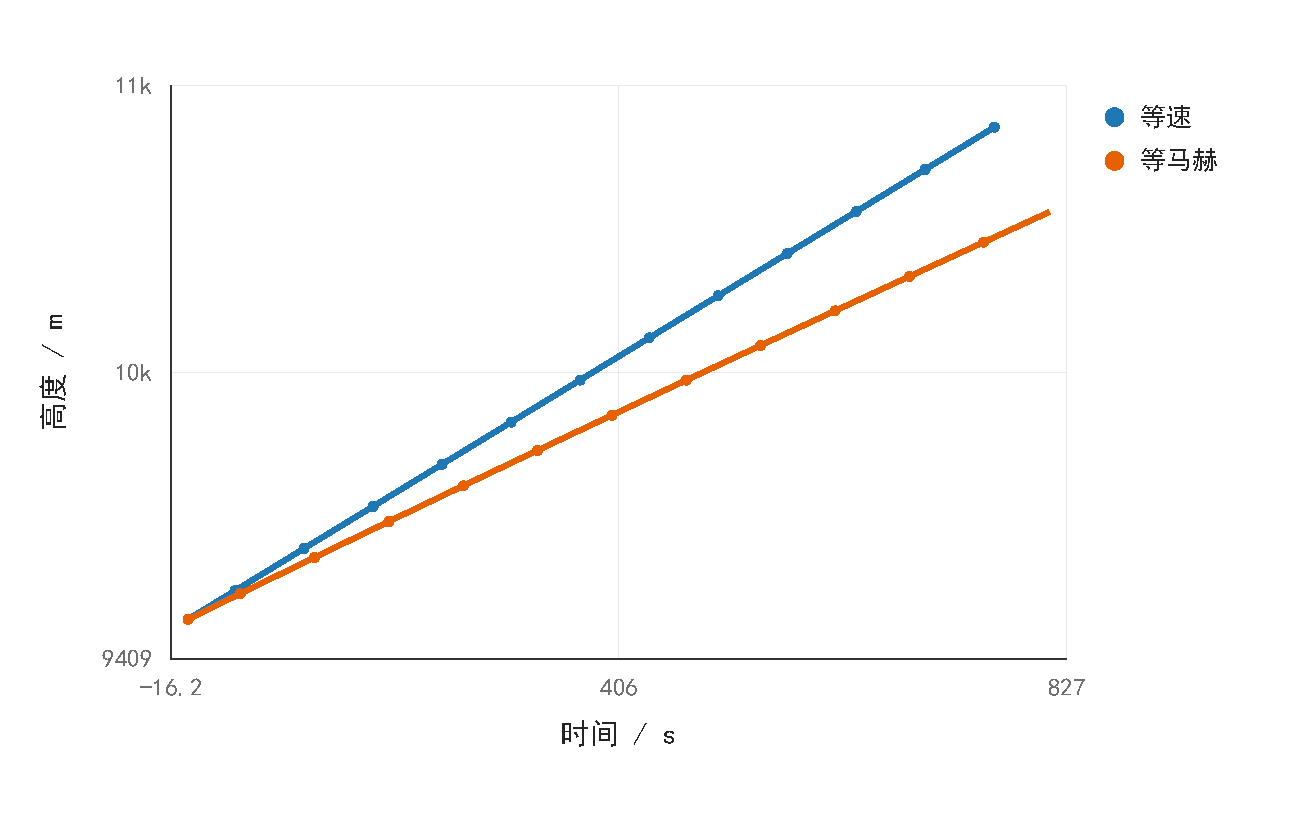
\includegraphics[width=\textwidth]{fig_v2_q1_height_time.pdf}
\par\smallskip{\small (a) 高度--时间剖面}
\end{minipage}
\hfill
\begin{minipage}[c]{0.49\textwidth}
\centering
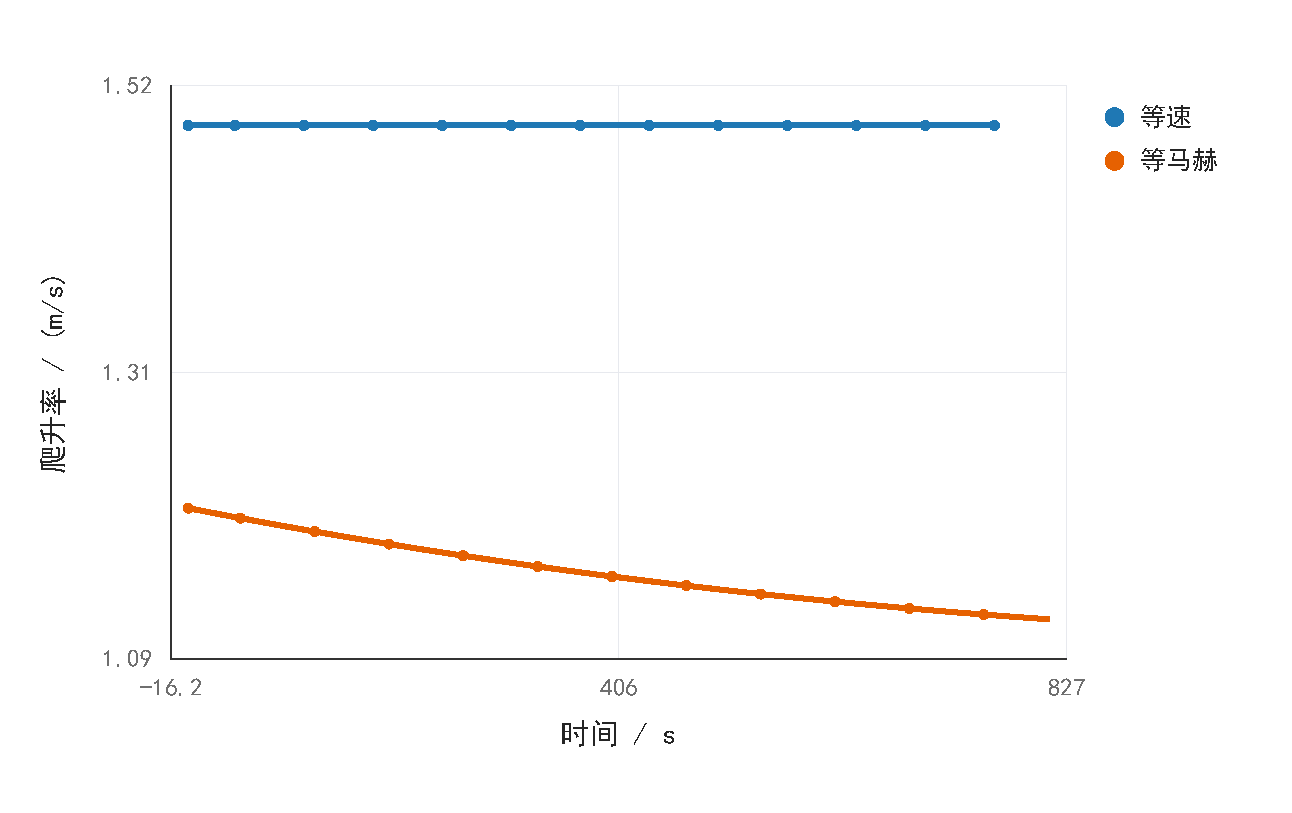
\includegraphics[width=\textwidth]{fig_v2_q1_climb_rate.pdf}
\par\smallskip{\small (b) 爬升率--时间剖面}
\end{minipage}
\caption{问题一两类经验策略的轨迹剖面对比}
\label{fig:q1_trajectory_pair}
\end{figure}

图 \ref{fig:q1_trajectory_pair} 表明，等速策略的高度曲线整体高于等马赫策略，并在 $761.917\ \mathrm{s}$ 时达到 $10637.065\ \mathrm{m}$；其爬升率也在全程保持较高水平。等马赫策略虽用时 $811.032\ \mathrm{s}$，但爬升率较低且随时间变化，终点高度仅为 $10437.818\ \mathrm{m}$。

\begin{figure}[H]
\centering
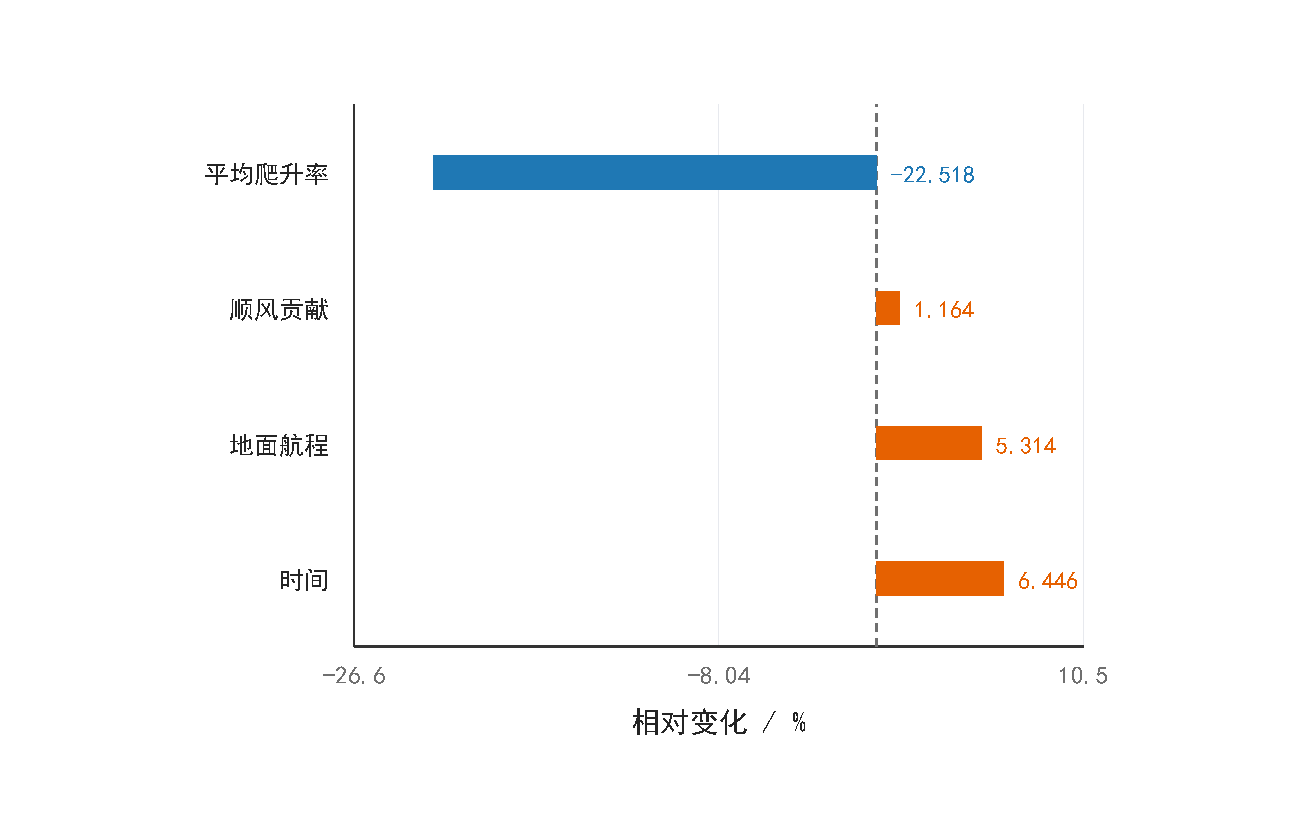
\includegraphics[width=0.86\textwidth]{fig_v2_q1_metric_comparison.pdf}
\caption{问题一等马赫策略相对等速策略的核心指标比例}
\label{fig:q1_metrics}
\end{figure}

由图 \ref{fig:q1_metrics} 可见，等马赫策略飞行时间约为等速策略的 $1.064$ 倍，地面航程约为 $1.053$ 倍，而平均爬升率仅约为 $0.775$ 倍；因此其航程增加主要来自时间延长和顺风累计，而不是更快爬升。

\subsubsection{高度和质量剖面解释}

等速策略下，$V=V_0$ 固定。随着飞机质量降低，为维持同一参考升力系数，空气密度也需按比例降低，因此飞机必须爬升到更高高度。指数密度模型使高度与质量满足对数关系 \eqref{eq:h_vs_m_constV}，所以在终止质量固定时最终高度由质量比直接决定。

等马赫策略下，$V=M_0a(h)$。在对流层近似中，声速随高度升高而下降，因此等马赫飞行意味着空速随高度升高而降低。升力平衡中的分母 $\rho(h)V^2$ 同时受密度下降和速度下降影响。由于 $V^2$ 的降低削弱了动压，飞机不需要达到等速策略那么高的高度即可满足固定 $C_L$ 的升力平衡关系。因此在本文模型下，等马赫策略最终高度低于等速策略。

这一机制也解释了爬升率差异。题面提示关注等马赫策略可能产生的爬升率优势，但在本文采用的闭合条件、风场和题设参数下，数值证据显示等速策略的平均爬升率更大。因此，本文将结论限定在当前模型和参数范围内：等马赫策略并未表现出更大的平均爬升率，其优势主要体现在更长飞行时间带来的航程增加。

\subsubsection{验证与诊断}

为检验数值解的可靠性，本文对初始条件、质量单调性、升力平衡、能量方程、步长敏感性、无风/有风对比和极端状态物理合理性进行了检查。验证结果见表 \ref{tab:validation}。

\begin{table}[h]
\centering\caption{问题一数值解验证结果}\label{tab:validation}
\begin{tabular}{lcc}\toprule
检查项 & 等速策略 & 等马赫策略 \\
\midrule
初始条件误差 & $0$ & $0$ \\
质量单调性 & 通过 & 通过 \\
最大升力平衡相对残差 & $0$ & $0$ \\
最大能量方程相对残差 & $9.72\times 10^{-17}$ & $9.95\times 10^{-17}$ \\
步长敏感性：最终时间 & $3.18\times 10^{-12}$ & $2.61\times 10^{-12}$ \\
步长敏感性：最终航程 & $6.69\times 10^{-10}$ & $7.57\times 10^{-10}$ \\
步长敏感性：平均爬升率 & $6.22\times 10^{-15}$ & $3.77\times 10^{-15}$ \\
\bottomrule
\end{tabular}
\end{table}

由表 \ref{tab:validation} 可知，两种策略均满足质量单调下降、升力平衡和能量方程约束，残差远低于 $10^{-6}$ 的设定阈值；步长减半或加倍后，最终时间、最终航程和平均爬升率的变化均保持在极小量级，说明该一维质量积分模型在当前参数下对积分步长不敏感。

\subsubsection{灵敏度分析}

本文进一步考察推力燃油消耗系数和速度偏离惩罚系数对结果的影响。

将 $c_T$ 降低一个数量级至 $2.8\times 10^{-5}$ 时，等速策略飞行时间增至 $8295.569\ \mathrm{s}$，等马赫策略飞行时间增至 $8624.642\ \mathrm{s}$；但两策略最终高度仍分别保持为 $10637.065\ \mathrm{m}$ 和 $10437.818\ \mathrm{m}$。这说明在当前闭合条件下，最终高度主要由升力平衡和终止质量决定，而时间尺度对燃油消耗系数高度敏感。

对 $\beta$ 作 $\pm 10\%$、$\pm 20\%$ 扰动时，两种策略最终高度同样保持不变，但飞行时间、航程和平均爬升率发生变化。表 \ref{tab:sensitivity} 给出了 $\beta$ 扰动下的结果。

\begin{table}[h]
\centering\caption{$\beta$ 扰动下的策略指标变化}\label{tab:sensitivity}
\begin{tabular}{lcccc}\toprule
扰动 & \multicolumn{2}{c}{等速策略} & \multicolumn{2}{c}{等马赫策略} \\
\cmidrule(lr){2-3} \cmidrule(lr){4-5}
 & 总时间/s & 平均爬升率/(m$\cdot$s$^{-1}$) & 总时间/s & 平均爬升率/(m$\cdot$s$^{-1}$) \\
\midrule
$-20\%$ & 773.762 & 1.469527 & 817.141 & 1.147682 \\
$-10\%$ & 767.798 & 1.480943 & 814.073 & 1.152007 \\
标称值 & 761.917 & 1.492374 & 811.032 & 1.156327 \\
$+10\%$ & 756.117 & 1.503821 & 808.017 & 1.160641 \\
$+20\%$ & 750.397 & 1.515283 & 805.029 & 1.164949 \\
\bottomrule
\end{tabular}
\end{table}

由表 \ref{tab:sensitivity} 可知，$\beta$ 增大时，速度偏离惩罚加重，燃油消耗率增大，导致在相同终止质量下飞行时间缩短；反之 $\beta$ 减小时飞行时间延长。该结果表明速度惩罚系数主要通过改变燃油消耗率影响时间和航程，而不改变由 $C_L=C_{L,\mathrm{ref}}$ 与终止质量决定的高度终点。

\section{问题二模型的建立与求解}

\subsection{固定几何路径与路径积分口径}

问题二的关键是把大气修正的影响从固定终止质量口径中分离出来。本文固定问题一等速策略得到的几何路径 $h_{\mathrm{ref}}(x)$ 与真空速路径
\begin{equation}
V_{\mathrm{ref}}(x)=240\ \mathrm{m/s},
\end{equation}
在每种大气场景中重新计算升力系数、阻力、推力需求和油耗率。为保证所有温差场景在同一航程下均满足 $m(t_f)\geq 62000\ \mathrm{kg}$，先分别计算各场景沿参考路径达到 $62000\ \mathrm{kg}$ 的航程，再取其中最短者作为共同可行航程：
\begin{equation}
X_{\mathrm{ref}}=189781.310\ \mathrm{m}.
\label{eq:q2_Xref}
\end{equation}

沿固定路径，地速为
\begin{equation}
V_g(x)=V_{\mathrm{ref}}+W(h_{\mathrm{ref}}(x)).
\end{equation}
燃油流率仍采用
\begin{equation}
q_f(x)=c_T T_{\mathrm{req}}(x)\left[1+\beta(V_{\mathrm{ref}}-V_{\mathrm{opt}})^2\right].
\label{eq:q2_fuel_flow}
\end{equation}
由于 $V_{\mathrm{ref}}$ 固定，速度偏离惩罚项在路径上为常数。路径域质量方程为
\begin{equation}
\frac{dm}{dx}=-\frac{q_f(x)}{V_g(x)}.
\label{eq:q2_dmdx}
\end{equation}
故共同航程下的总油耗为
\begin{equation}
J=\int_0^{X_{\mathrm{ref}}}\frac{q_f(x)}{V_g(x)}\,dx
=m_0-m(X_{\mathrm{ref}}).
\label{eq:q2_path_integral}
\end{equation}

\subsection{标准大气与常温偏差静力修正}

标准 ISA 给出了对流层内温度、压力随高度变化的基准关系\cite{icao_atmos}，本文写为
\begin{equation}
T_0(h)=T_{\mathrm{sl}}-L_T h,\qquad
p_0(h)=p_{\mathrm{sl}}\left(\frac{T_0(h)}{T_{\mathrm{sl}}}\right)^{g/(R L_T)}.
\end{equation}
密度与声速为
\begin{equation}
\rho_0(h)=\frac{p_0(h)}{R T_0(h)},\qquad
a_0(h)=\sqrt{\gamma R T_0(h)}.
\end{equation}

对于常温偏差 $\Delta T$，本文不采用只改温度而保持 ISA 压力不变的简化处理，而采用满足静力平衡的非标准大气修正：
\begin{equation}
T_\Delta(h)=T_{\mathrm{sl}}+\Delta T-L_T h,
\label{eq:q2_T_delta}
\end{equation}
\begin{equation}
p_\Delta(h)=p_{\mathrm{sl}}
\left(\frac{T_{\mathrm{sl}}+\Delta T-L_T h}{T_{\mathrm{sl}}+\Delta T}\right)^{g/(R L_T)},
\label{eq:q2_p_delta}
\end{equation}
其中程序实现中采用与式 \eqref{eq:q2_T_delta} 对应的幂律压力剖面并检查
\begin{equation}
\frac{|dp_\Delta/dh+\rho_\Delta g|}{\rho_\Delta g}<10^{-4}.
\end{equation}
密度与声速由
\begin{equation}
\rho_\Delta(h)=\frac{p_\Delta(h)}{R T_\Delta(h)},\qquad
a_\Delta(h)=\sqrt{\gamma R T_\Delta(h)}
\end{equation}
给出。

在同一几何路径上，升力平衡要求
\begin{equation}
C_L(x)=\frac{2m(x)g}{\rho_\Delta(h_{\mathrm{ref}}(x))V_{\mathrm{ref}}^2S},
\label{eq:q2_CL}
\end{equation}
阻力为
\begin{equation}
D(x)=\frac{1}{2}\rho_\Delta(h_{\mathrm{ref}}(x))V_{\mathrm{ref}}^2S
\left(C_{D0}+kC_L^2(x)\right).
\label{eq:q2_drag}
\end{equation}
考虑小角度爬升功率项，所需推力写为
\begin{equation}
T_{\mathrm{req}}(x)=D(x)+\frac{m(x)g}{V_{\mathrm{ref}}}\frac{dh_{\mathrm{ref}}}{dt},
\qquad
\frac{dh_{\mathrm{ref}}}{dt}=\frac{dh_{\mathrm{ref}}}{dx}V_g(x).
\label{eq:q2_thrust}
\end{equation}

式 \eqref{eq:q2_CL}--\eqref{eq:q2_thrust} 表明，大气连续分布通过密度直接进入升力系数、诱导阻力和总阻力；温度和压力通过静力平衡共同决定密度；声速在当前固定真空速模型中主要用于马赫数诊断。也就是说，本问温差修正对油耗的影响主要经由密度和阻力传递，而不是直接改变速度路径。若后续引入等马赫策略、波阻或马赫相关发动机效率，声速才会进一步进入油耗率模型。

\begin{figure}[H]
\centering
\begin{minipage}[c]{0.48\textwidth}
\centering
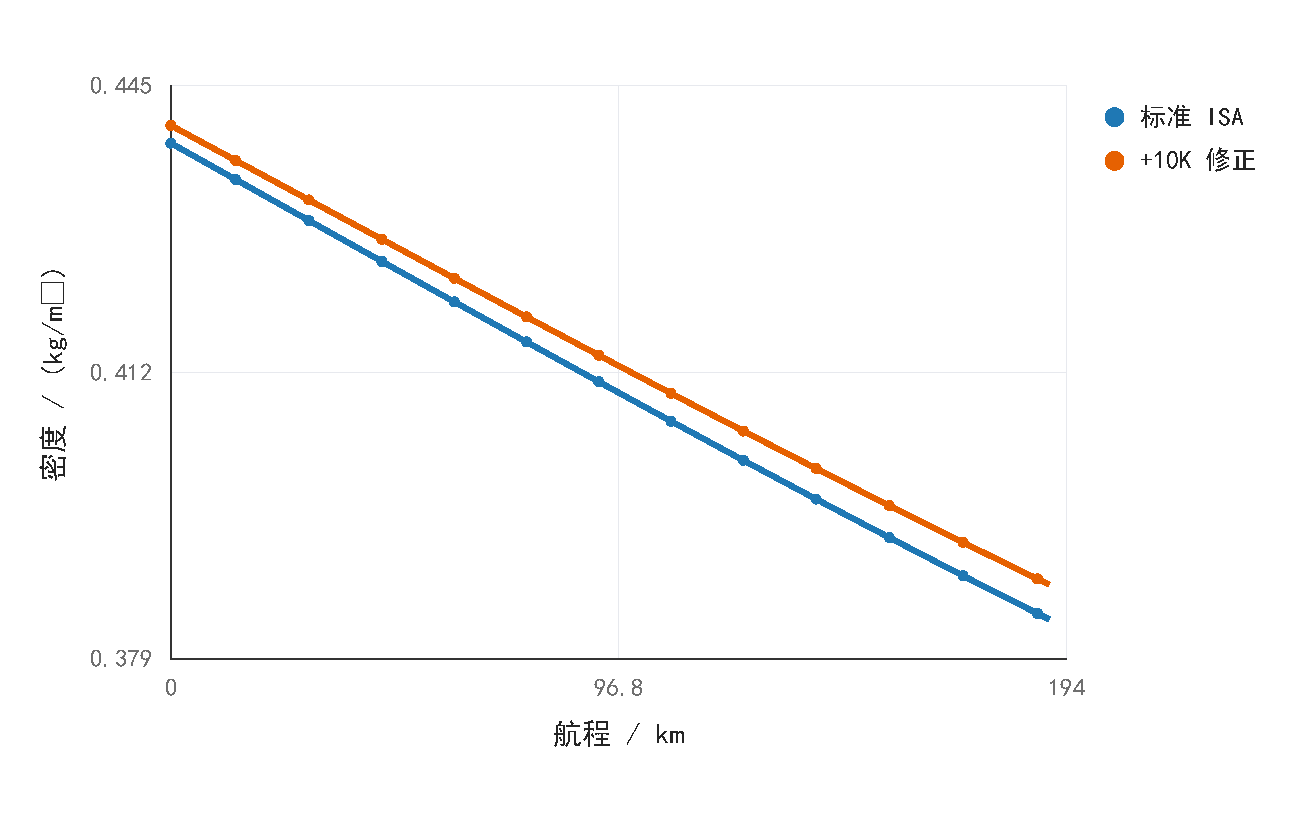
\includegraphics[width=\textwidth]{fig_v2_q2_density_correction.pdf}
\par\smallskip{\small (a) 沿程密度修正}
\end{minipage}
\hfill
\begin{minipage}[c]{0.48\textwidth}
\centering
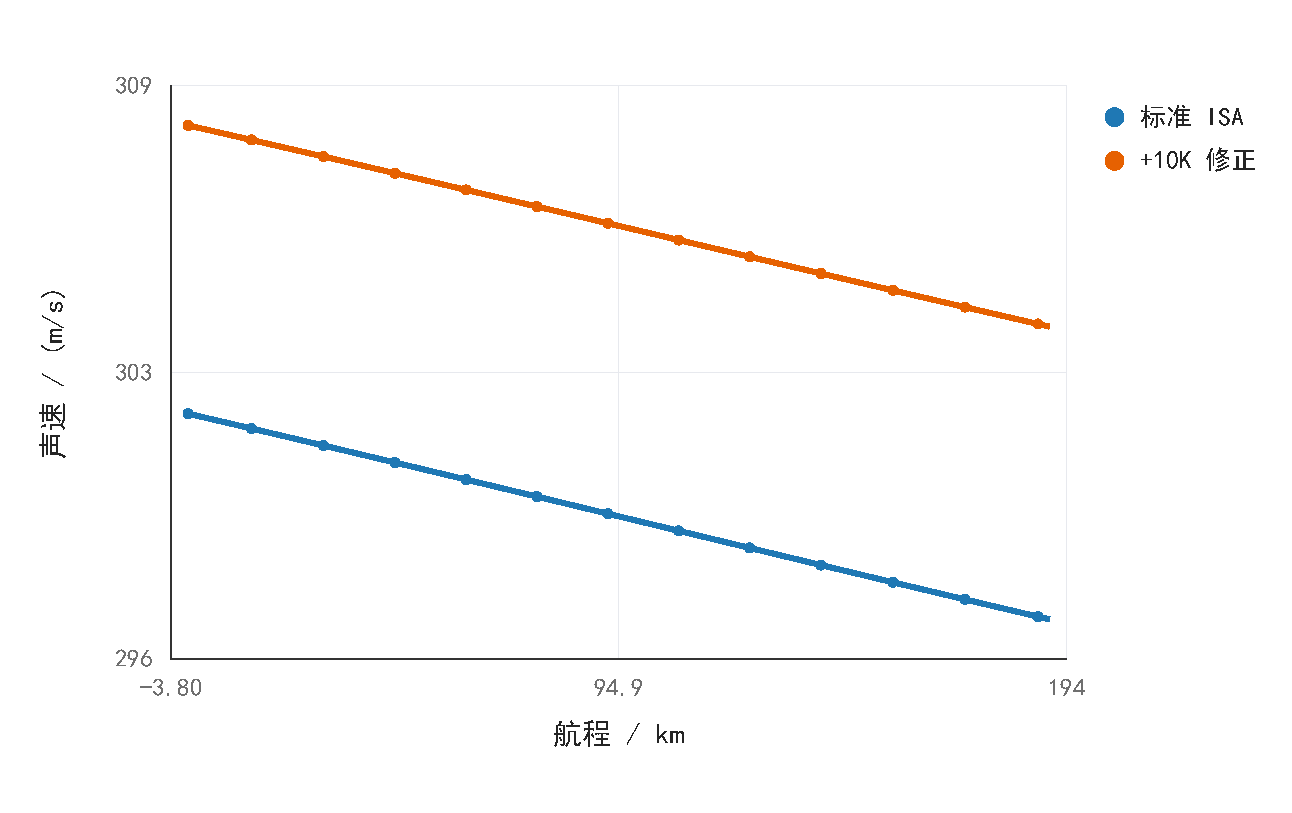
\includegraphics[width=\textwidth]{fig_v2_q2_sound_speed_correction.pdf}
\par\smallskip{\small (b) 沿程声速修正}
\end{minipage}
\caption{问题二温差静力修正对关键大气量的影响}
\label{fig:q2_atmosphere_pair}
\end{figure}

图 \ref{fig:q2_atmosphere_pair} 表明，$+10\ \mathrm{K}$ 静力修正并不是只改变温度，而是同时通过压力和状态方程改变沿程密度，并通过温度改变声速诊断。在同一真空速下，密度改变会影响升力系数和诱导阻力；若后续引入等马赫策略或马赫相关发动机效率，声速变化还会进一步进入油耗率模型。

\subsection{标准 ISA 与温差修正结果}

共同可行航程固定为 $189781.310\ \mathrm{m}$ 后，温差修正的影响主要通过沿程燃油率差异逐步累积。由于两种大气口径下瞬时燃油率曲线非常接近，本文直接展示累计油耗差，如图 \ref{fig:q2_fuel_accumulation} 所示。

\begin{figure}[H]
\centering
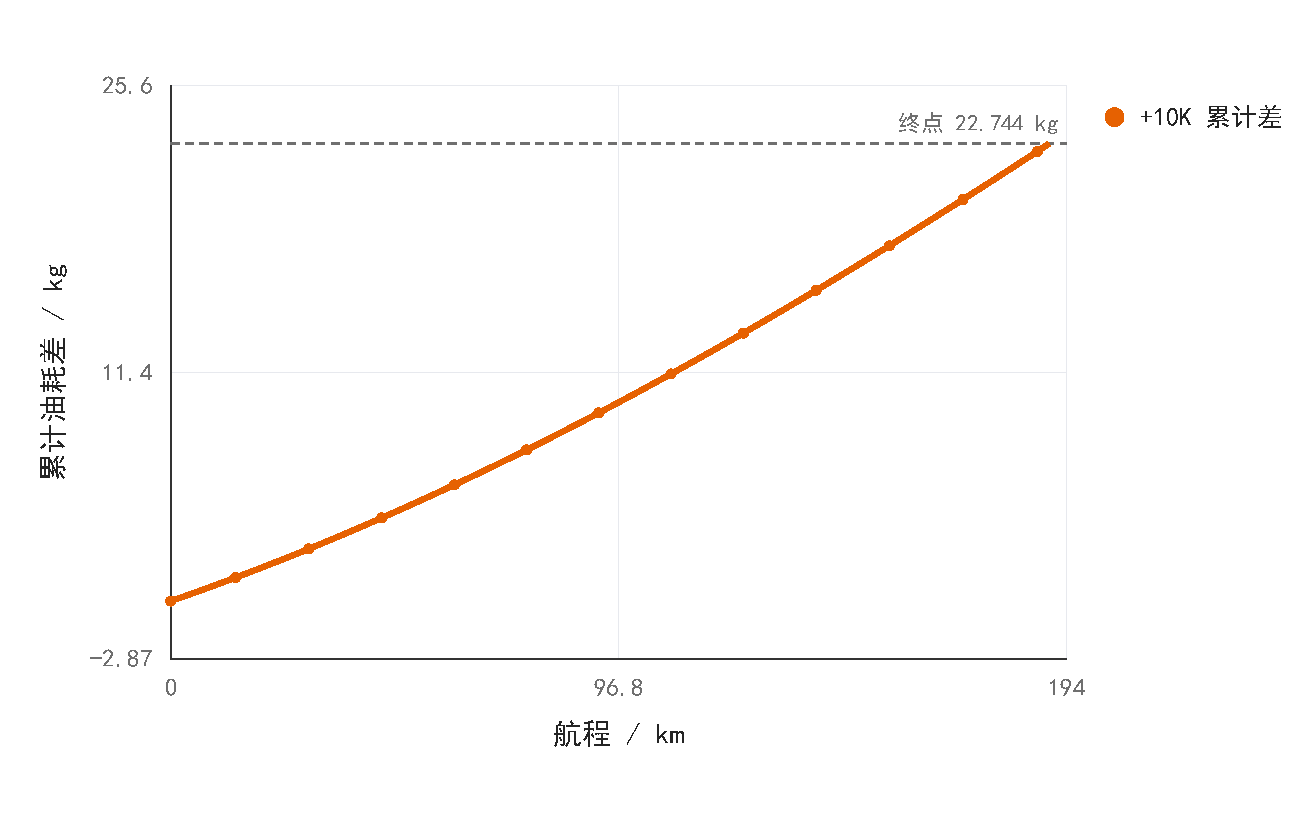
\includegraphics[width=0.86\textwidth]{fig_v2_q2_fuel_accumulation.pdf}
\caption{问题二 $+10\ \mathrm{K}$ 修正相对标准 ISA 的累计油耗差}
\label{fig:q2_fuel_accumulation}
\end{figure}

由图 \ref{fig:q2_fuel_accumulation} 可见，油耗差并非来自某个局部突变，而是随航程平滑累积；终点累计差为 $22.744\ \mathrm{kg}$。标准 ISA 总油耗为 $10427.256\ \mathrm{kg}$，$+10\ \mathrm{K}$ 场景总油耗为 $10450.000\ \mathrm{kg}$，精确汇总见表 \ref{tab:q2_fuel_summary}。

\begin{table}[htpb]
\centering
\caption{问题二共同可行航程下的燃油消耗结果}
\label{tab:q2_fuel_summary}
\begin{tabular}{lrrc}\toprule
指标 & 标准 ISA & $+10\ \mathrm{K}$ 静力修正 & 单位 \\
\midrule
共同可行航程 & 189781.310 & 189781.310 & m \\
飞行时间 & 721.753 & 721.753 & s \\
总油耗 & 10427.256 & 10450.000 & kg \\
终点质量 & 62022.744 & 62000.000 & kg \\
单位距离油耗 & 0.054944 & 0.055063 & kg/m \\
相对标准大气变化 & 0.000 & 0.218 & \% \\
\bottomrule
\end{tabular}
\end{table}

表 \ref{tab:q2_fuel_summary} 说明，在固定几何路径和固定真空速下，升温会改变同一高度上的密度水平，进而影响升力系数和诱导阻力结构，使总油耗略有增加。$+10\ \mathrm{K}$ 静力修正比标准 ISA 多消耗
\begin{equation}
10450.000-10427.256=22.744\ \mathrm{kg},
\end{equation}
相对增加 $0.218\%$。

\subsection{温差灵敏度分析}

为判断温度偏差能否忽略，本文计算 $\Delta T\in\{-10,-5,-2,0,2,5,10\}\ \mathrm{K}$ 七个场景。图 \ref{fig:q2_temperature_sensitivity} 先展示趋势：随温度偏差由负转正，总油耗单调增加，终点质量相应单调降低。

\begin{figure}[H]
\centering
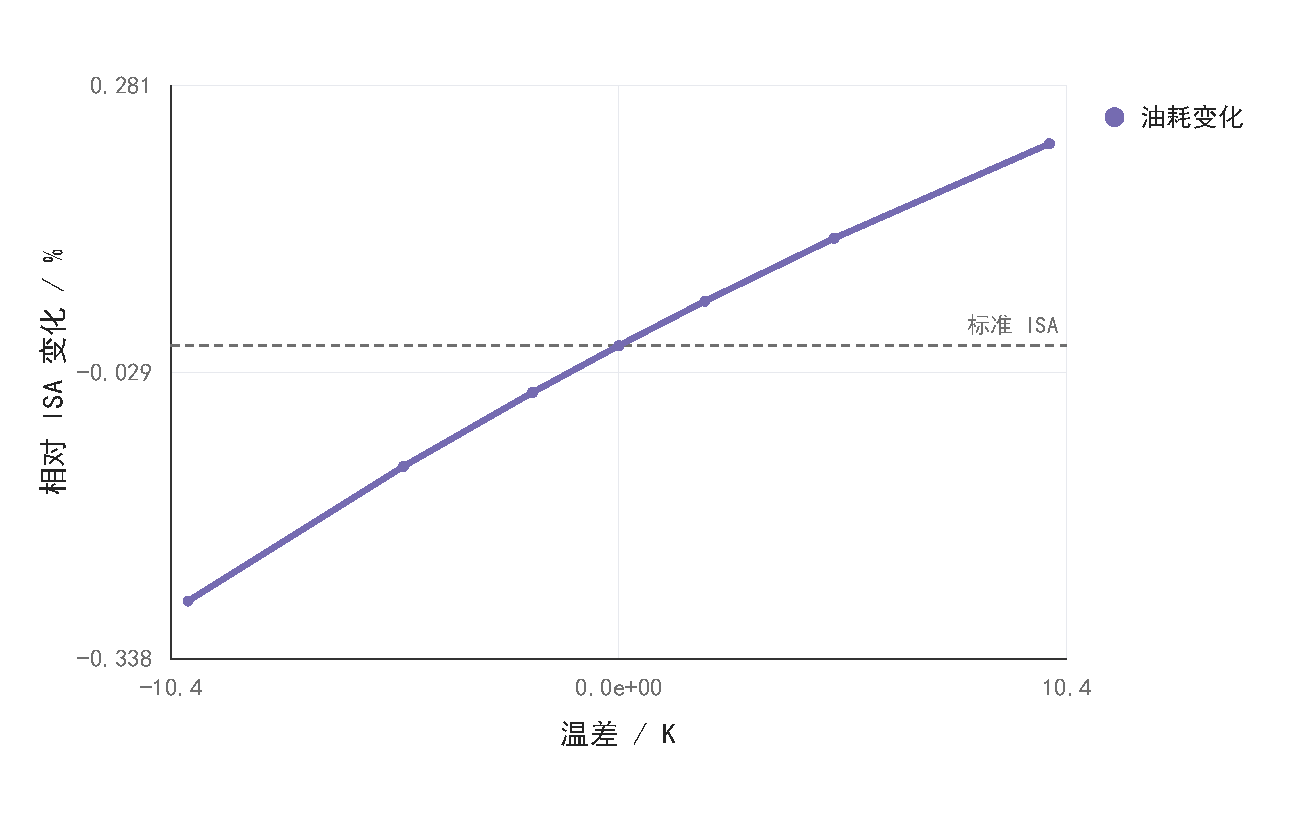
\includegraphics[width=0.86\textwidth]{fig_v2_q2_temperature_sensitivity.pdf}
\caption{问题二常温偏差对总油耗的灵敏度}
\label{fig:q2_temperature_sensitivity}
\end{figure}

图 \ref{fig:q2_temperature_sensitivity} 显示，温差对油耗的影响方向明确但幅度较小。对应的精确数值列于表 \ref{tab:q2_temp_sensitivity}：在 $\Delta T=-10\ \mathrm{K}$ 时总油耗降至 $10398.507\ \mathrm{kg}$；在 $\Delta T=10\ \mathrm{K}$ 时总油耗增至 $10450.000\ \mathrm{kg}$，终点质量恰好降到 $62000.000\ \mathrm{kg}$。

\begin{table}[htpb]
\centering
\caption{常温偏差下的总油耗灵敏度}
\label{tab:q2_temp_sensitivity}
\begin{tabular}{rrrr}\toprule
$\Delta T$ / K & 总油耗 / kg & 终点质量 / kg & 相对 ISA 变化 / \% \\
\midrule
-10 & 10398.507 & 62051.493 & -0.276 \\
-5 & 10413.660 & 62036.340 & -0.130 \\
-2 & 10422.001 & 62027.999 & -0.050 \\
0 & 10427.256 & 62022.744 & 0.000 \\
2 & 10432.271 & 62017.729 & 0.048 \\
5 & 10439.350 & 62010.650 & 0.116 \\
10 & 10450.000 & 62000.000 & 0.218 \\
\bottomrule
\end{tabular}
\end{table}

由表 \ref{tab:q2_temp_sensitivity} 和图 \ref{fig:q2_temperature_sensitivity} 可见，在当前固定 q1 几何路径、固定真空速和题设参数下，$|\Delta T|\leq10\ \mathrm{K}$ 时总油耗变化均小于 $0.3\%$。若所需计算精度约为 $1\%$，这类常温偏差可作为二阶修正处理；若需要千分级油耗评估，或温度偏差超过上述范围，则应采用非标准大气修正。

\subsection{验证与诊断}

问题二从状态一致性、大气物理一致性和数值积分一致性三个方面进行验证。所有场景的初始高度、速度和质量与题设一致，固定航程误差为 $0\ \mathrm{m}$，终点质量均不低于 $62000\ \mathrm{kg}$；路径位于对流层内，静力平衡残差约为 $10^{-10}$ 量级；时间积分、路径积分和最终质量亏损的最大差异约为 $0.0016\ \mathrm{kg}$，低于 $0.05\ \mathrm{kg}$ 阈值。步长加倍后标准 ISA 总油耗变化约为 $3.65\times10^{-8}\ \mathrm{kg}$，说明问题二路径积分结果对离散步长不敏感。

\section{问题三模型的建立与求解}

问题三在问题一、二基础上把经验策略推广为最优控制问题。求解分两步：先用航程域直接配点获得连续可行轨迹，再以 reduced-control shooting 进行最终燃油最小化，并通过独立连续验证确认结果的物理一致性。直接配点用于先获得满足路径约束的可行初值，shooting 则保留连续动力学积分的检验优势，这一组合与轨迹优化文献中“先转录、再验证”的思路一致\cite{hargraves,betts}。有风条件下的最优控制结果在问题四中给出。

\subsection{建模口径与边界条件}

问题三要求在给定初始飞行状态下，以总燃油消耗最小为目标，确定高度--速度联合变化规律\cite{cook,cots2022}。为避免固定终止质量导致目标函数退化，本文采用固定航程和固定终点飞行状态的口径：固定共同航程
\[
X_f=189781.310\ \mathrm{m},
\]
并约束终点高度和速度分别与问题一等速策略终点一致，即
\[
h(t_f)=10577.124\ \mathrm{m},\qquad V(t_f)=240\ \mathrm{m/s}.
\]
终点质量 $m(t_f)$ 作为优化结果保留，燃油最省等价于最大化终点质量。该口径既避免了目标退化，也避免通过降低终点机械能换取表观节油。

\subsubsection{最优控制模型}

取状态变量为 $x(t),h(t),V(t),m(t)$，控制变量为推力 $T(t)$ 与航迹角 $\gamma(t)$。目标函数写为
\begin{equation}
\max\ m(t_f),
\qquad \text{等价于}\qquad
\min\ J=m_0-m(t_f).
\label{eq:q3_objective}
\end{equation}
动力学约束为
\begin{equation}
\begin{cases}
\dot x=V\cos\gamma+W(h),\\[3pt]
\dot h=V\sin\gamma,\\[3pt]
\dot V=\dfrac{T-D-mg\sin\gamma}{m},\\[8pt]
\dot m=-c_T T\left[1+\beta\left(V-V_{\mathrm{opt}}\right)^2\right],
\end{cases}
\label{eq:q3_dynamics}
\end{equation}
其中阻力 $D$ 仍由升阻模型 $D=\tfrac12\rho V^2S(C_{D0}+kC_L^2)$ 给出，升力系数由纵向力平衡或小航迹角近似确定。边界条件为
\begin{equation}
\begin{cases}
x(0)=0,\quad h(0)=h_0,\quad V(0)=V_0,\quad m(0)=m_0,\\
x(t_f)=X_f,\quad h(t_f)=10577.124\ \mathrm{m},\quad V(t_f)=240\ \mathrm{m/s},\\
m(t_f)\geq62000\ \mathrm{kg}.
\end{cases}
\label{eq:q3_boundary}
\end{equation}
工程约束包括高度、速度、马赫数、推力、升力系数和爬升角边界：
\begin{equation}
h_{\min}\leq h\leq h_{\max},\quad
V_{\min}\leq V\leq V_{\max},\quad
M\leq M_{\max},\quad
0\leq T\leq T_{\max},\quad
C_{L,\min}\leq C_L\leq C_{L,\max}.
\label{eq:q3_path_constraints}
\end{equation}

\subsubsection{必要条件与求解路径}

间接法主要用于解释最优性条件。根据 Pontryagin 极大值原理，构造哈密顿量\cite{pontryagin}
\begin{equation}
H=\lambda_x(V\cos\gamma+W(h))+\lambda_hV\sin\gamma
\lambda_V\frac{T-D-mg\sin\gamma}{m}
-\lambda_m c_TT\left[1+\beta(V-V_{\mathrm{opt}})^2\right],
\label{eq:q3_hamiltonian}
\end{equation}
由庞特里亚金极大值原理可写出协态方程、控制驻值条件和终端横截条件。由于间接法对初值敏感，本文数值上采用直接配点法，将连续轨迹离散为节点变量并转化为非线性规划问题\cite{hargraves,betts}；得到离散解后，再用原微分方程独立重积分，检查终点高度、速度、质量和路径约束是否仍满足。

\subsection{航程域直接配点与可行初值构造}

为避免直接把有风基线误当作无风可行初值，本文首先在固定等速几何路径上分别重算配置风场和无风场景。结果见表 \ref{tab:q3_baseline_feasibility}。配置风场下，固定路径终点质量为 $62022.744\ \mathrm{kg}$，满足质量约束；无风条件下同一路径终点质量仅为 $61163.474\ \mathrm{kg}$，质量缺口约 $836.526\ \mathrm{kg}$，说明必须重新构造无风可行轨迹。

\begin{table}[htbp]
\centering
\caption{问题三固定路径可行性预检查}
\label{tab:q3_baseline_feasibility}
\begin{tabular}{lrrrr}\toprule
风场场景 & 航程/m & 终点质量/kg & 总油耗/kg & 是否满足质量约束 \\
\midrule
配置风场 & 189781.310 & 62022.744 & 10427.256 & 是 \\
无风 & 189781.310 & 61163.474 & 11286.526 & 否 \\
\bottomrule
\end{tabular}
\end{table}

表 \ref{tab:q3_baseline_feasibility} 的差异在图 \ref{fig:q3_feasibility_bridge} 中更直观：配置风场固定路径仅略高于质量下限，而无风固定路径明显落到下限以下；重新优化后，终端质量恢复到 $62107.186\ \mathrm{kg}$。因此，问题三的直接配点并非单纯追求节油，而是先解决无风条件下的可行性。

\begin{figure}[H]
\centering
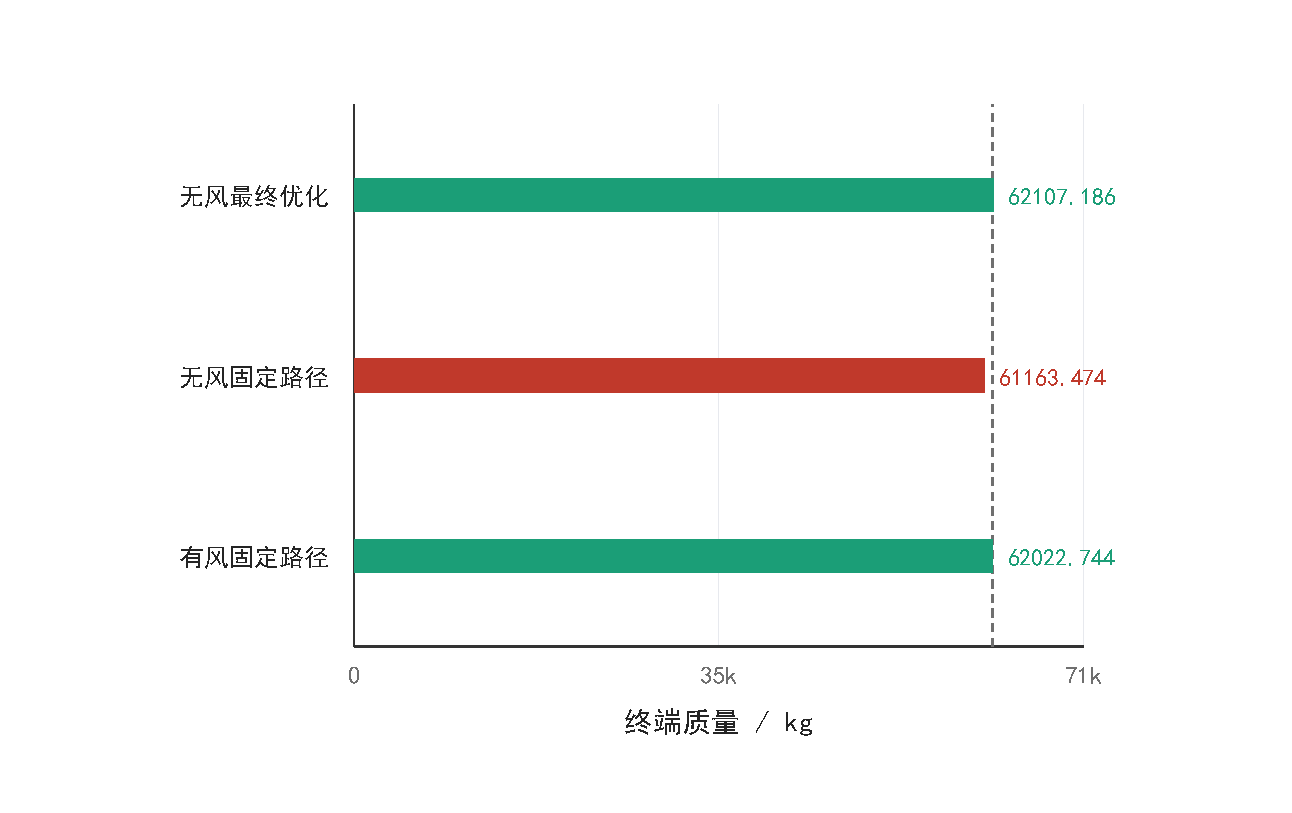
\includegraphics[width=0.86\textwidth]{fig_v2_q3_feasibility_bridge.pdf}
\caption{问题三固定路径可行性与最终优化终端质量对比}
\label{fig:q3_feasibility_bridge}
\end{figure}

进一步采用航程域直接配点法进行无风可行性求解。状态取 $(h,V,m,t)$，控制取 $(T,\gamma)$，用梯形配点离散式 \eqref{eq:q3_dynamics} 对应的航程域微分方程；大气模型采用 $C^1$ 温度平滑和静力压力积分，避免轨迹穿越 $11\ \mathrm{km}$ 层界时出现不可微问题。第一阶段不追求节油，只最小化终端质量松弛 $s$；当 $s$ 降至数值零后，再用独立微分方程重积分检查连续轨迹是否满足终点和路径约束。

可行性求解的作用是为最终燃油优化提供连续可行的初值。结果显示，最终优化采用该初值并在 $61\to121\to241$ 节点逐级加密中保持稳定。表 \ref{tab:q3_mesh_convergence} 给出三个网格层级下的最终优化结果：节点数由 $61$ 增至 $241$ 时，总油耗始终稳定在 $10342.81\ \mathrm{kg}$ 附近，$N=121$ 与 $N=241$ 的差异仅为 $3.28\times10^{-4}\ \mathrm{kg}$，说明最终结果不是某一离散网格的偶然输出。

\begin{table}[htbp]
\centering
\caption{问题三无风最终优化网格稳定性诊断}
\label{tab:q3_mesh_convergence}
\begin{tabular}{rrrrr}\toprule
节点数 & 总油耗/kg & 终点质量/kg & 终点时间/s & 优化迭代次数 \\
\midrule
61  & 10342.805 & 62107.195 & 805.681 & 22 \\
121 & 10342.815 & 62107.185 & 805.680 & 11 \\
241 & 10342.814 & 62107.186 & 805.679 & 13 \\
\bottomrule
\end{tabular}
\end{table}

由表 \ref{tab:q3_mesh_convergence} 可见，$N=61,121,241$ 三个网格的燃油差异集中在 $10^{-2}\ \mathrm{kg}$ 量级以内。图 \ref{fig:q3_grid_stability} 进一步显示三层网格的总油耗均稳定在 $10342.81\ \mathrm{kg}$ 附近，说明最终优化结果不是某一离散网格的偶然输出。

\begin{figure}[H]
\centering
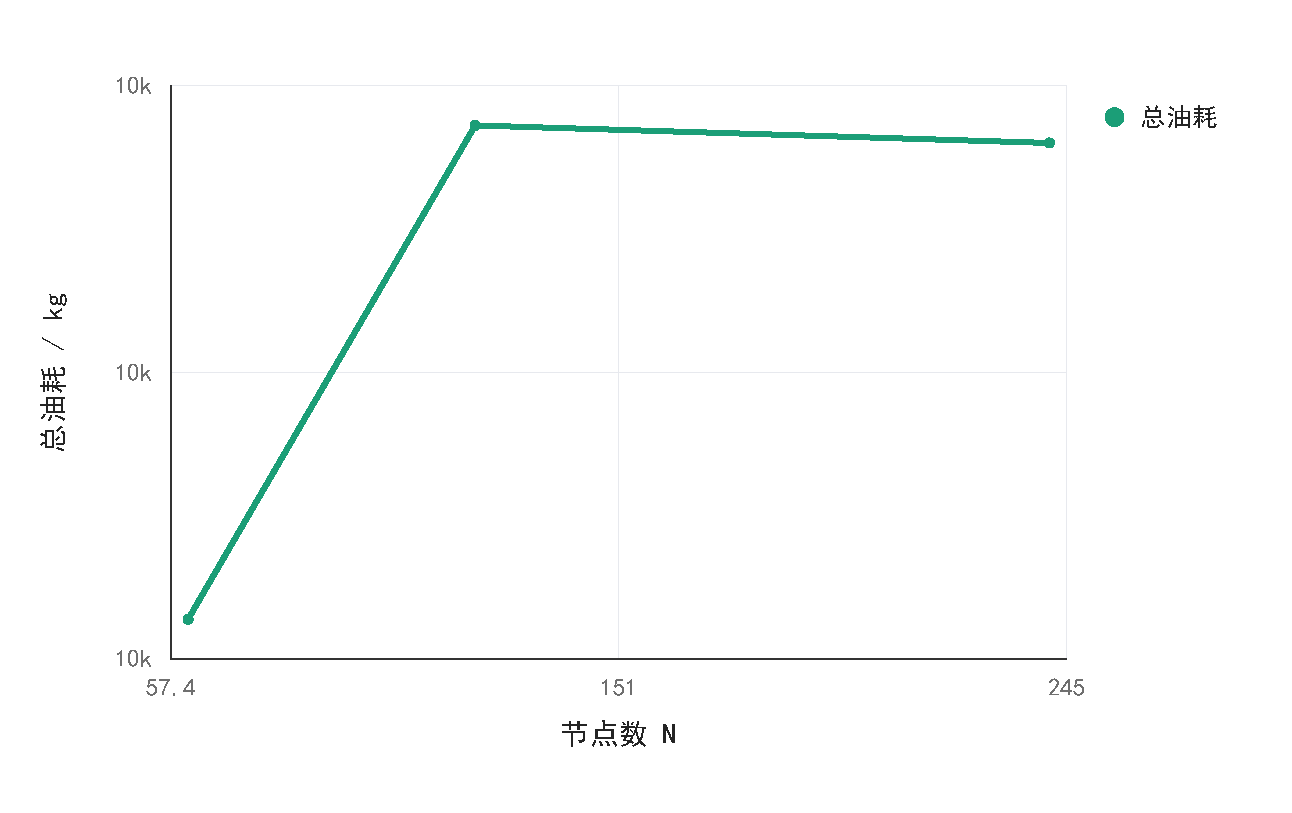
\includegraphics[width=0.82\textwidth]{fig_v2_q3_grid_stability.pdf}
\caption{问题三无风最终优化的网格稳定性}
\label{fig:q3_grid_stability}
\end{figure}

\subsection{无风最终燃油优化结果}

在可行初值轨迹基础上，本文进一步采用 reduced-control shooting 进行最终燃油优化。具体做法是将推力和航迹角用少量控制结点参数化，以可行性求解结果作为初始猜测，沿航程积分原连续动力学，并把终端高度、速度、质量下限和路径约束作为优化约束。该方法减少了直接配点中的大规模离散变量，使最终优化更接近连续动力学口径。有风条件下的扩展在问题四中给出。

最终轨迹的主要形态见图 \ref{fig:q3_final_trajectory}。高度曲线先快速爬升，随后在巡航中段贴近 $12000\ \mathrm{m}$ 上界；质量曲线则随航程单调下降，并在终点保留约 $107.186\ \mathrm{kg}$ 的质量余量。这一形态说明，高度上界在无风最终优化中接近活跃，终端质量约束则未被压到边界。

\begin{figure}[H]
\centering
\begin{minipage}[c]{0.48\textwidth}
\centering
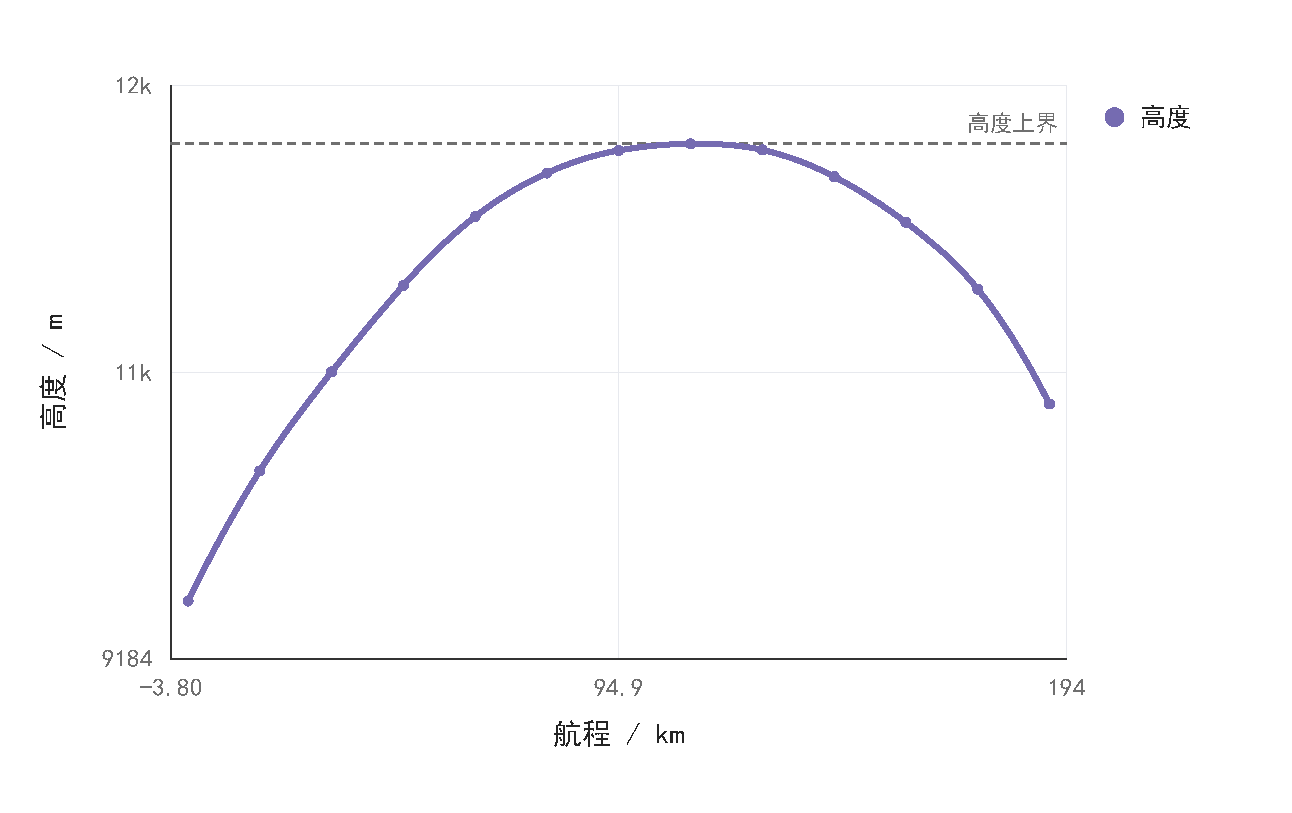
\includegraphics[width=\textwidth]{fig_v2_q3_state_corridor_height.pdf}
\par\smallskip{\small (a) 最终高度轨迹}
\end{minipage}
\hfill
\begin{minipage}[c]{0.48\textwidth}
\centering
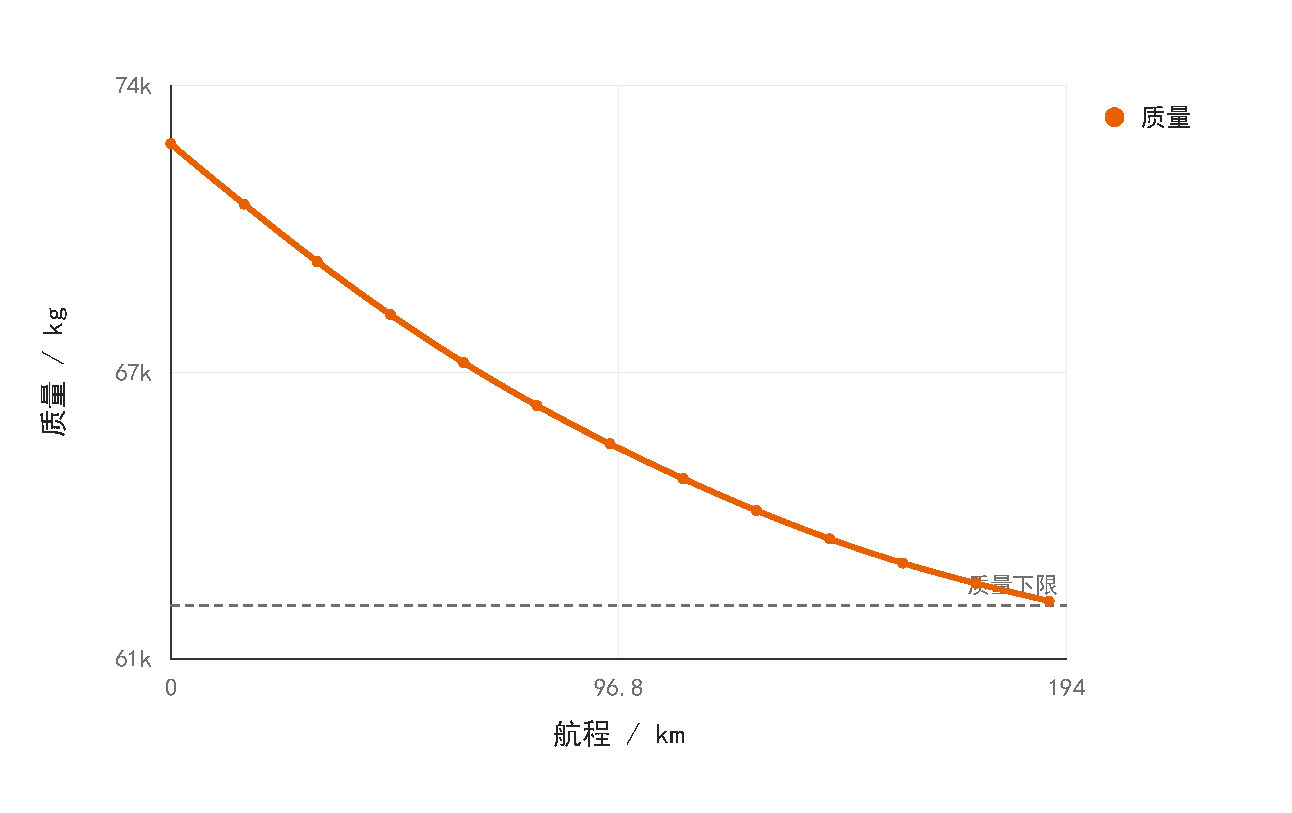
\includegraphics[width=\textwidth]{fig_v2_q3_state_corridor_mass.pdf}
\par\smallskip{\small (b) 最终质量轨迹}
\end{minipage}
\caption{问题三无风最终燃油优化的状态轨迹}
\label{fig:q3_final_trajectory}
\end{figure}

从数值上看，可行性候选燃油为 $10450.000\ \mathrm{kg}$，最终 reduced-control shooting 解降至 $10342.814\ \mathrm{kg}$，减少约 $107.186\ \mathrm{kg}$；由于终端时间比 $t_f/t_{\mathrm{base}}=1.01887$，该收益并非来自明显拉长飞行时间。表 \ref{tab:q3_final_optimal} 给出无风最终优化的核心状态和约束余量。

\begin{table}[htbp]
\centering
\caption{问题三无风最终燃油优化核心结果}
\label{tab:q3_final_optimal}
\begin{tabular}{lrrc}\toprule
指标 & 数值 & 约束或对照 & 单位 \\
\midrule
总燃油消耗 & 10342.814 & 可行性候选为 10450.000 & kg \\
终端质量 & 62107.186 & 下限 62000.000 & kg \\
终端时间 & 805.679 & $t_f/t_{\mathrm{base}}=1.01887$ & s \\
最大高度 & 11999.960 & 上界 12000.000 & m \\
空速范围 & 234.029--240.000 & 满足包线 & m/s \\
推力范围 & 19634.093--73083.701 & 满足包线 & N \\
最大马赫数 & 0.808261 & 满足约束 & -- \\
\bottomrule
\end{tabular}
\end{table}

\begin{figure}[H]
\centering
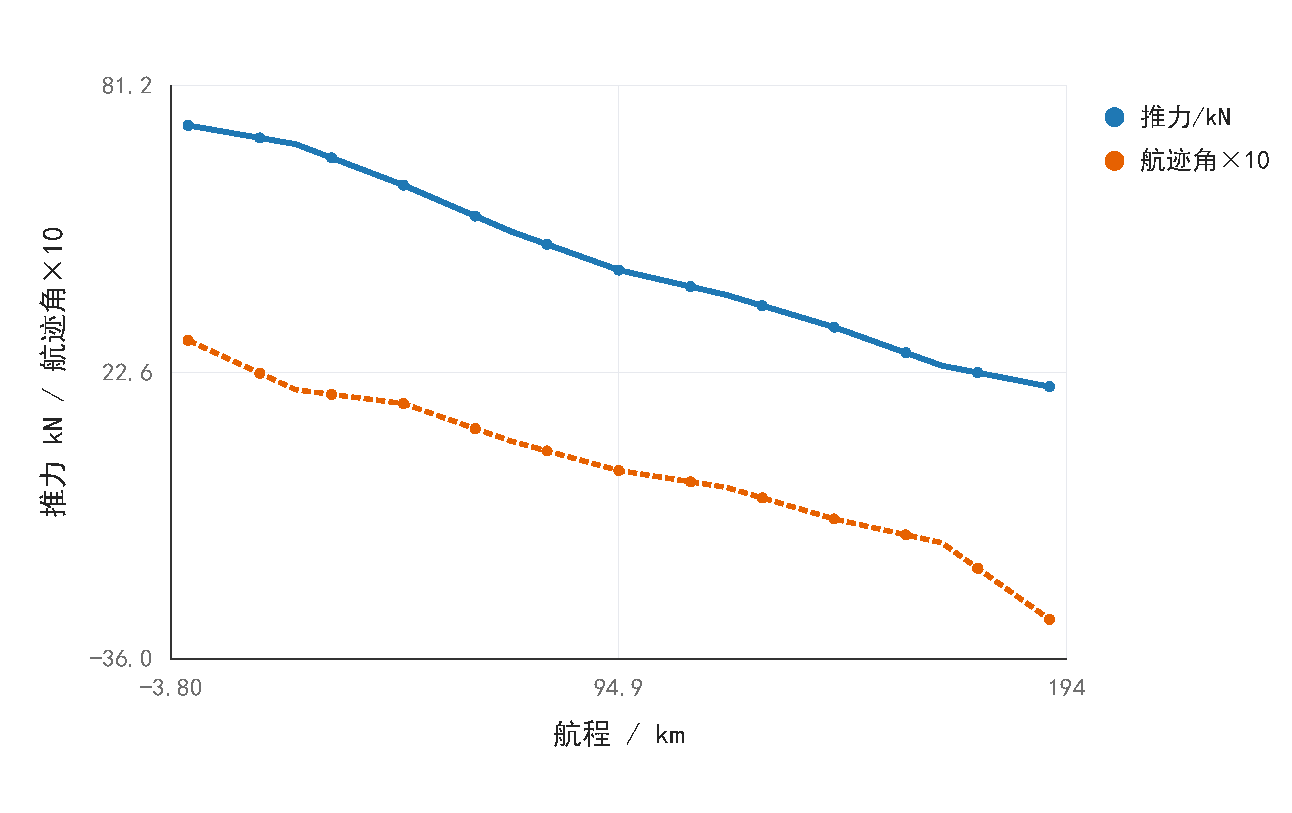
\includegraphics[width=0.86\textwidth]{fig_v2_q3_control_schedule.pdf}
\caption{问题三无风最终燃油优化的控制量形态}
\label{fig:q3_final_control}
\end{figure}

图 \ref{fig:q3_final_control} 显示，最终优化中的推力范围为 $19.634$--$73.084\ \mathrm{kN}$，没有触及零推力或怠速推力下界；航迹角围绕小角度变化，与小航迹角准稳态假设相容。该结果也解释了后文怠速推力扰动对当前无风解影响较弱的原因。

\subsection{连续验证与局部灵敏度边界}

为确认最终优化不是离散网格上的偶然结果，本文对 reduced-control shooting 解进行独立连续验证。验证内容包括原微分方程重积分、燃油恒等式、网格目标差异、多初值一致性、时间约束和连续路径约束。结果见表 \ref{tab:q3_final_validation}。

\begin{table}[htbp]
\centering
\caption{问题三无风最终优化连续验证结果}
\label{tab:q3_final_validation}
\begin{tabular}{lrrc}\toprule
验证项目 & 数值 & 阈值 & 状态 \\
\midrule
终端速度重积分误差/(m/s) & $1.71\times10^{-5}$ & $10^{-3}$ & 通过 \\
终端高度重积分误差/m & $3.62\times10^{-4}$ & $10^{-1}$ & 通过 \\
燃油恒等式残差/kg & $8.58\times10^{-5}$ & $5.0\times10^{-2}$ & 通过 \\
网格目标差异/kg & $3.28\times10^{-4}$ & $1.0$ & 通过 \\
多初值目标范围/kg & $4.27\times10^{-2}$ & $1.0$ & 通过 \\
连续约束违反 & $0$ & $0$ & 通过 \\
\bottomrule
\end{tabular}
\end{table}

\begin{figure}[H]
\centering
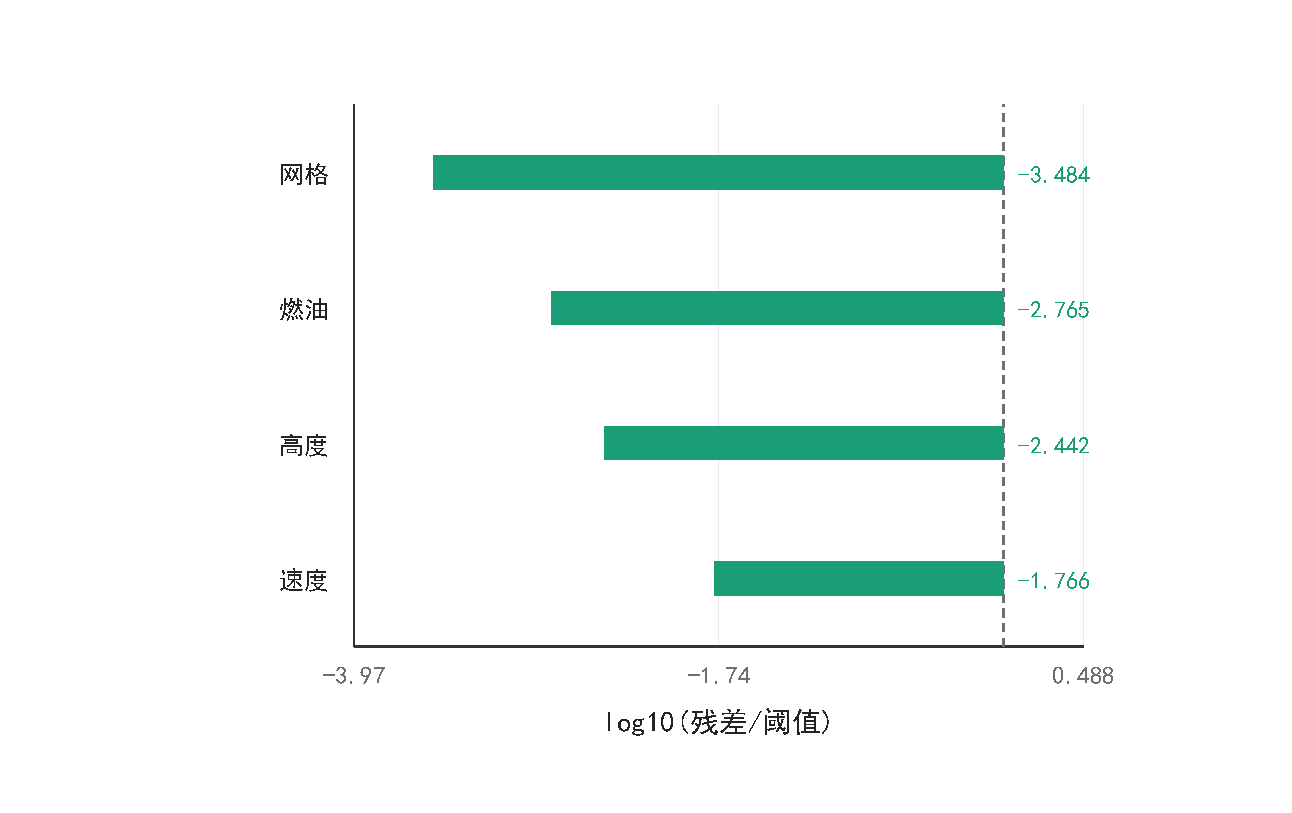
\includegraphics[width=0.8\textwidth]{fig_v2_q3_validation_dashboard.pdf}
\caption{问题三无风最终优化验证残差相对阈值}
\label{fig:q3_validation_summary}
\end{figure}

由表 \ref{tab:q3_final_validation} 和图 \ref{fig:q3_validation_summary} 可见，所有关键残差均低于阈值，且验证状态为 passed。其中终端速度重积分误差仅为 $1.71\times10^{-5}\ \mathrm{m/s}$，燃油恒等式残差为 $8.58\times10^{-5}\ \mathrm{kg}$，说明无风最终燃油优化结果具有连续动力学一致性。

局部灵敏度方面，当前仓库还给出了高度上界和怠速推力的初步重优化结果。$h_{\max}=12500\ \mathrm{m}$ 的局部计算得到燃油约 $10334.057\ \mathrm{kg}$，比 $12000\ \mathrm{m}$ 上界情形低约 $8.757\ \mathrm{kg}$，提示高度上界可能是影响无风最优油耗的活跃约束；但该灵敏度当前基于 $N=121$ 局部重优化，且部分状态标记为 failed，因此只能作为趋势提示。怠速推力扰动的油耗变化不超过 $0.01\ \mathrm{kg}$，与最终轨迹最小推力约 $19.634\ \mathrm{kN}$、高于怠速下界的事实一致；但同样不宜写成全局结论。

\section{问题四模型的建立与求解}

问题四在前三问基础上形成综合计算框架，任务是将等速经验策略、固定路径油耗积分和有风最优控制结果放在同一评价口径下比较，并对速度偏离惩罚系数等关键参数进行重新求解式灵敏度分析。已有有风轨迹优化研究通常把风速视为随高度或空间变化的外部场，并在燃油、时间或排放目标下求解受约束最优控制问题\cite{park2015,jafarimoghaddam2023}。本文以问题一等速巡航爬升剖面和问题二共同航程油耗为基线，在问题三无风最优轨迹基础上引入有风航程域最优控制，采用 reduced-control shooting 进行局部优化。

\subsection{有风最优控制模型}

问题四沿用问题三的动力学方程 \eqref{eq:q3_dynamics}，但将风场 $W(h)$ 显式保留在地速表达式中，这与有风飞行轨迹优化中把沿程风速纳入地速方程的处理一致\cite{park2015,jafarimoghaddam2023}：
\begin{equation}
V_g=V\cos\gamma+W(h),\qquad W(h)=20+3\times 10^{-5}(h-10000)^2\ \mathrm{m/s}.
\label{eq:q4_wind}
\end{equation}
航程域动力学通过将时间域方程除以 $V_g$ 获得，并增加 $dt/dx=1/V_g$。目标函数仍为固定航程下最小化燃油消耗：
\begin{equation}
\min\ J=m_0-m(t_f),\qquad X_f=189781.310\ \mathrm{m}.
\label{eq:q4_objective}
\end{equation}
终端高度和速度约束与问题三一致，即 $h(t_f)=10577.124\ \mathrm{m}$、$V(t_f)=240\ \mathrm{m/s}$。边界条件与路径约束沿用式 \eqref{eq:q3_boundary}--\eqref{eq:q3_path_constraints}。

\subsection{求解策略}

有风最优控制以问题三无风最终燃油优化轨迹作为初始猜测，采用航程域 reduced-control shooting：将推力和航迹角用 5 个分段线性控制结点参数化，状态由原连续动力学沿航程积分，终端高度、速度和质量下限作为优化约束。该方法降低了直接配点中的大规模离散变量，使最终优化更接近连续动力学口径。优化采用序列二次规划方法，最大迭代 300 次，输出节点 41 个。

\subsection{有风最优与等速基线对比}

表 \ref{tab:q4_strategy_compare} 给出等速基线与有风局部优化策略在固定共同航程 $189781.310\ \mathrm{m}$ 下的核心指标对比。等速基线复用问题二标准 ISA 固定航程结果，燃油消耗 $10427.256\ \mathrm{kg}$；有风局部优化轨迹燃油消耗 $9863.840\ \mathrm{kg}$，节省 $563.416\ \mathrm{kg}$，相对节省比例 $5.403\%$。为避免两个万公斤量级油耗柱形掩盖差异，图 \ref{fig:q4_strategy_savings} 直接突出固定航程下的节油幅度。

\begin{figure}[H]
\centering
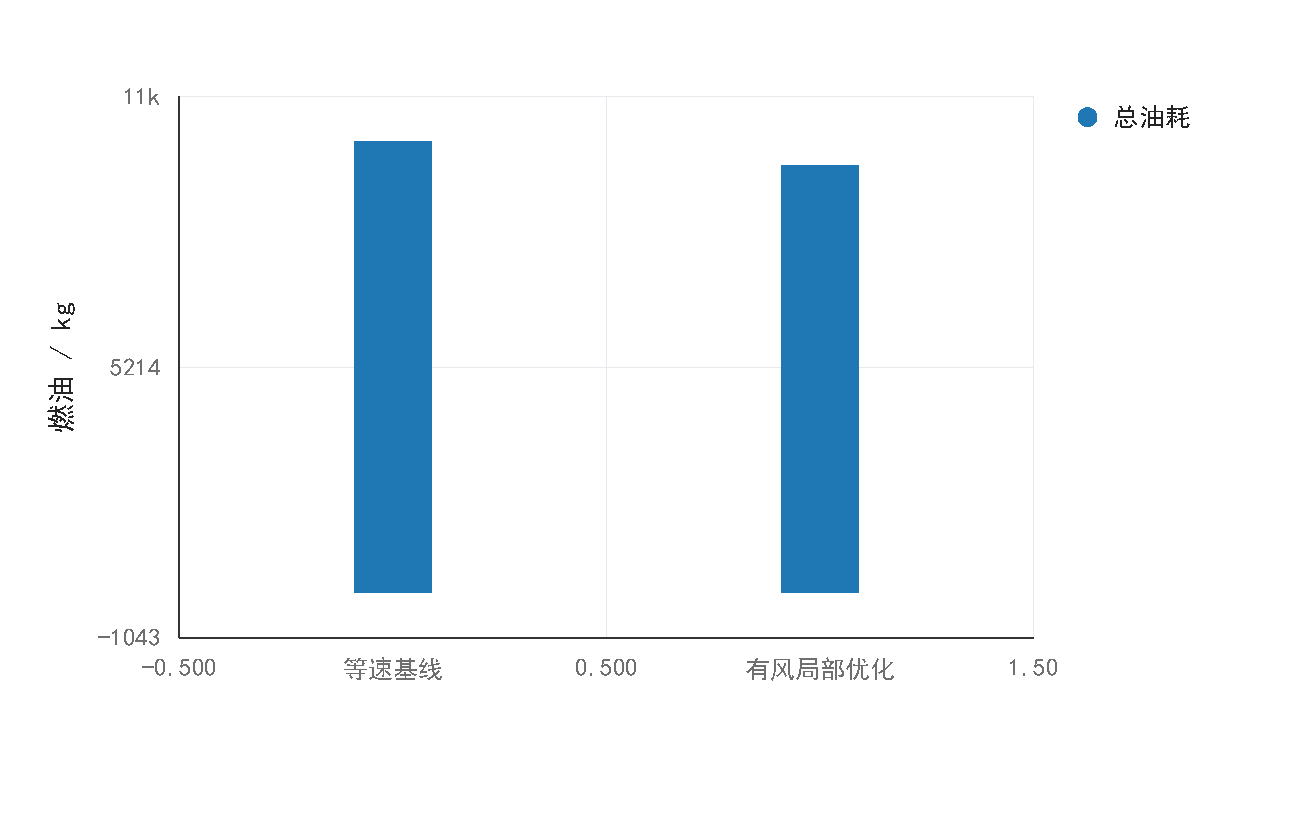
\includegraphics[width=0.82\textwidth]{fig_v2_q4_strategy_savings.pdf}
\caption{问题四固定共同航程下的燃油消耗对比}
\label{fig:q4_strategy_savings}
\end{figure}

\begin{table}[htbp]
\centering\caption{问题四等速基线与有风局部优化策略对比}\label{tab:q4_strategy_compare}
\begin{tabular}{lrrc}\toprule
指标 & 等速基线 & 有风局部优化 & 单位 \\
\midrule
固定共同航程 & 189781.310 & 189781.310 & m \\
总燃油消耗 & 10427.256 & 9863.840 & kg \\
终端质量 & 62022.744 & 62586.160 & kg \\
飞行时间 & 721.753 & 733.758 & s \\
燃油节省 & -- & 563.416 (5.403\%) & kg \\
\bottomrule
\end{tabular}
\end{table}

由表 \ref{tab:q4_strategy_compare} 和图 \ref{fig:q4_strategy_savings} 可知，在固定航程和配置风场下，有风局部优化轨迹比等速基线少消耗约 $5.4\%$ 的燃油。有风优化轨迹飞行时间略长（$733.758\ \mathrm{s}$ 对 $721.753\ \mathrm{s}$），表明优化器通过调整高度和速度剖面，更充分地利用了顺风条件降低推力需求，而不是简单缩短飞行时间。

\subsection{有风最优轨迹形态分析}

有风局部优化轨迹的节油并非来自缩短飞行时间，而是来自高度、速度和推力剖面的重新分配。图 \ref{fig:q4_profile_pair} 将高度剖面与控制剖面并排给出：优化轨迹在巡航中段低于等速基线，末段再回到终端高度约束附近。

\begin{figure}[H]
\centering
\begin{minipage}[c]{0.48\textwidth}
\centering
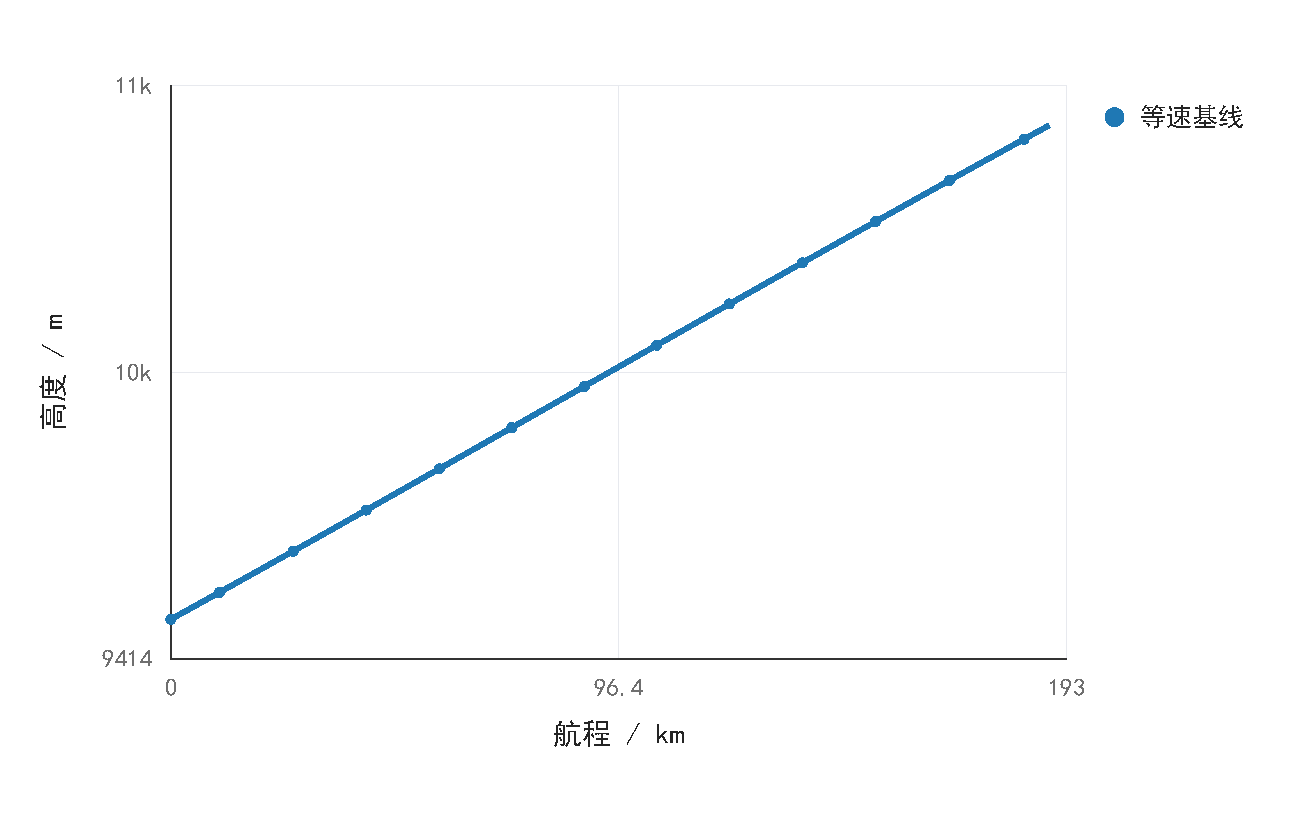
\includegraphics[width=\textwidth]{fig_v2_q4_height_profile_compare.pdf}
\par\smallskip{\small (a) 高度剖面对比}
\end{minipage}
\hfill
\begin{minipage}[c]{0.48\textwidth}
\centering
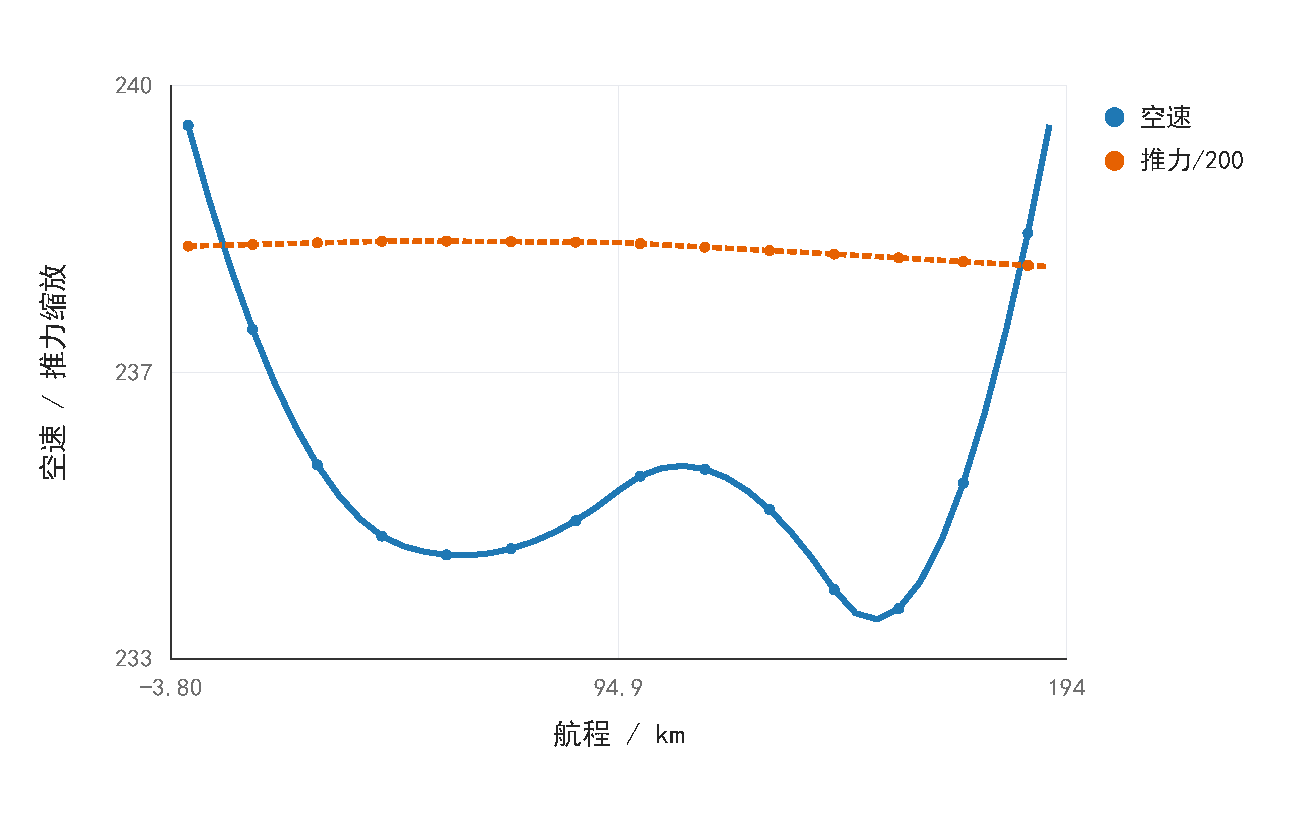
\includegraphics[width=\textwidth]{fig_v2_q4_control_profile.pdf}
\par\smallskip{\small (b) 有风优化控制剖面}
\end{minipage}
\caption{问题四有风局部优化轨迹形态}
\label{fig:q4_profile_pair}
\end{figure}

由图 \ref{fig:q4_profile_pair} 可见，有风优化轨迹在巡航中段高度低于等速基线，在终端附近爬升至与等速基线相近的高度。这种“先低后高”的剖面结构有利于在中段利用较低高度处较高的空气密度维持升力平衡；与之相配合，空速从 $240\ \mathrm{m/s}$ 略降至约 $234\ \mathrm{m/s}$ 后回升至终端值，推力维持在 $47.6$--$47.7\ \mathrm{kN}$ 的窄幅区间内。

\subsection{固定燃油口径下的航程估计}

为补充"航程变化"这一比较维度，本文在固定燃油预算 $10450\ \mathrm{kg}$（即问题一终止质量口径）下，以 $1.00$、$1.03$、$1.06$ 三个航程因子进行局部航程网格搜索。表 \ref{tab:q4_fixed_fuel_range} 给出结果。

\begin{table}[htbp]
\centering\caption{问题四固定燃油口径下的航程估计}\label{tab:q4_fixed_fuel_range}
\begin{tabular}{rrrr}\toprule
航程因子 & 试验航程/m & 燃油预算检查 & 状态 \\
\midrule
1.00 & 189781.310 & 通过 & 预算内 \\
1.03 & 195475.049 & 通过 & 预算内 \\
1.06 & 201168.189 & 通过（剩余 $49.393\ \mathrm{kg}$） & 预算内 \\
\bottomrule
\end{tabular}
\end{table}

三个航程因子下终端质量均不低于 $62000\ \mathrm{kg}$，$1.06$ 因子仍剩余 $49.393\ \mathrm{kg}$ 燃油，因此 $201168.189\ \mathrm{m}$ 是当前局部网格的可达航程下界估计。图 \ref{fig:q4_fixed_fuel_range} 将三档航程试验按固定燃油预算口径画出，强调该结果是“预算内下界”而非最大航程证明。

\begin{figure}[H]
\centering
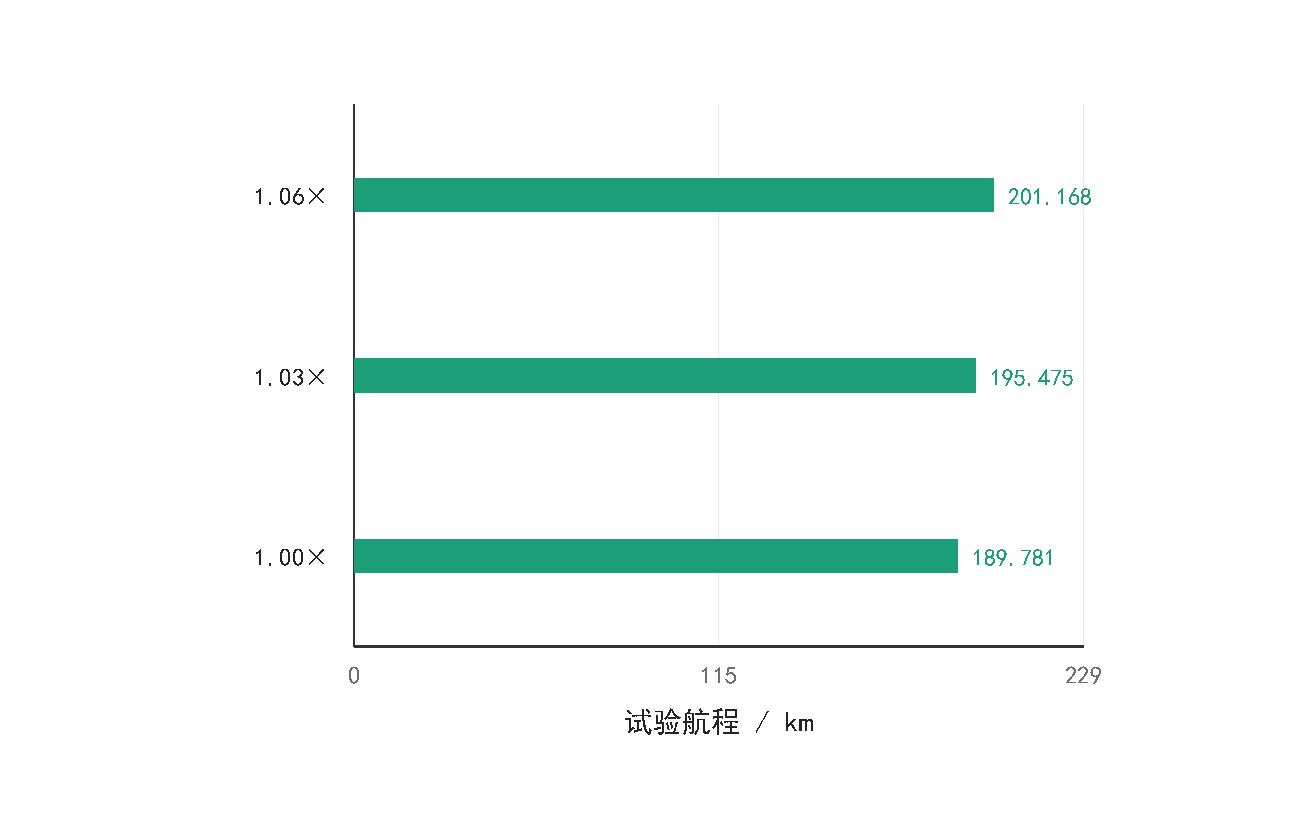
\includegraphics[width=0.82\textwidth]{fig_v2_q4_fixed_fuel_range.pdf}
\caption{问题四固定燃油预算下的可达航程下界估计}
\label{fig:q4_fixed_fuel_range}
\end{figure}

相对固定共同航程 $189781.310\ \mathrm{m}$，可达航程增量下界为 $11386.879\ \mathrm{m}$，增量比例约 $6.0\%$。由于航程搜索未括住不可行或超预算上界，该数值为下界估计而非严格最大航程。

\subsection{速度偏离惩罚系数灵敏度}

$\beta$ 灵敏度采用逐场景重新求解方式，每个扰动因子下均从标称解出发进行有风 reduced-control shooting 重优化，而非在标称轨迹上后验重算。表 \ref{tab:q4_beta_sensitivity} 给出五档结果。

\begin{table}[htbp]
\centering\caption{问题四 $\beta$ 扰动灵敏度}\label{tab:q4_beta_sensitivity}
\begin{tabular}{rrrrr}\toprule
$\beta$ 因子 & 总燃油/kg & 相对变化/kg & 终端质量/kg & 验证状态 \\
\midrule
0.8 & 9849.724 & $-14.116$ & 62600.276 & 通过 \\
0.9 & 9852.888 & $-10.953$ & 62597.112 & 通过 \\
1.0（标称） & 9863.840 & 0.000 & 62586.160 & 通过 \\
1.1 & 9869.462 & $+5.621$ & 62580.538 & 通过 \\
1.2 & 9870.070 & $+6.230$ & 62579.930 & 通过 \\
\bottomrule
\end{tabular}
\end{table}

由表 \ref{tab:q4_beta_sensitivity} 可见，$\beta$ 降低 $20\%$ 时局部可行解燃油减少 $14.116\ \mathrm{kg}$（$0.143\%$），$\beta$ 增大 $20\%$ 时燃油增加 $6.230\ \mathrm{kg}$（$0.063\%$）。五档扰动均通过独立微分方程重积分、终端状态和燃油恒等式验证。但非标称场景优化未达到最优终止条件，因此该结果仅支持局部可行敏感性描述，不宜外推为严格最优敏感性结论。

\begin{figure}[H]
\centering
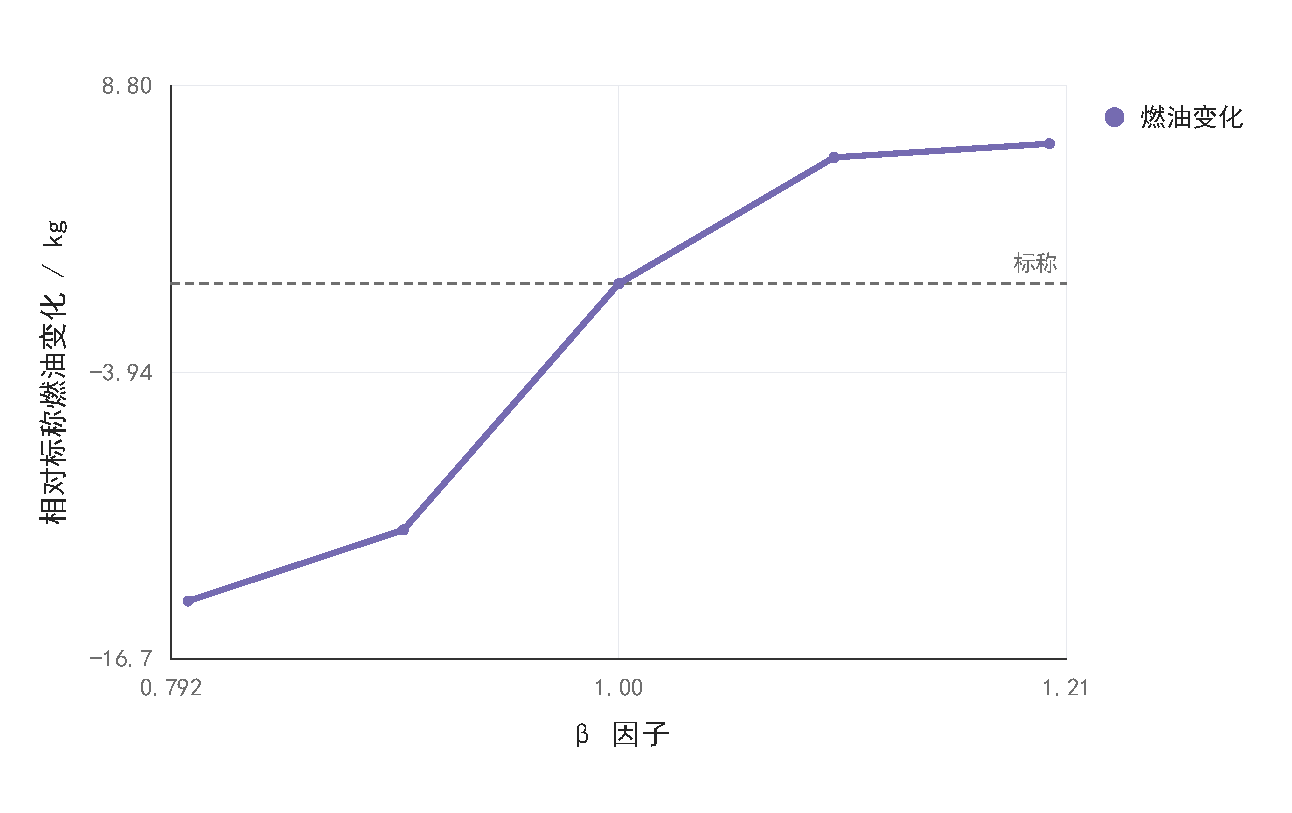
\includegraphics[width=0.84\textwidth]{fig_v2_q4_beta_sensitivity.pdf}
\caption{问题四 $\beta$ 扰动灵敏度响应}
\label{fig:q4_beta_sensitivity}
\end{figure}

图 \ref{fig:q4_beta_sensitivity} 直观显示，$\beta$ 在标称值附近变化时燃油响应近似线性，且整体波动幅度不超过 $0.15\%$，说明在当前参数化和求解口径下，有风局部优化轨迹对速度偏离惩罚系数不太敏感。

\subsection{模型扩展方向}

为进一步拓展模型的工程适用性，本文提出两个扩展框架。

\textbf{扩展一：温度实时修正。} 将问题二中的标准 ISA 大气调用替换为实时温度偏移或实测温度剖面 $T(h,t)$，在每次求阻力和燃油率前重新进行静力压力积分，使密度和声速与温度场自洽。该扩展需要沿航程温度偏差廓线或机载/预报温度场数据，验证方式为对比问题二静力温差场景下的修正结果。

\textbf{扩展二：发动机安装损失。} 将理想指令推力 $T$ 替换为有效推力 $\eta_{\mathrm{inst}}(h,M,T)T$，并引入安装燃油流率乘子 $\phi_{\mathrm{inst}}(h,M)$，推力边界仍作用于指令推力。该扩展需要发动机安装效率表（随高度、马赫数和推力设定变化），验证方式为在 $\eta_{\mathrm{inst}}=1.00$ 时回归到当前无损失结果，并在 $\{0.95,0.98,1.00\}$ 三档下比较终端约束和燃油影响。

\section{灵敏度分析}

本节汇总问题一至问题四的参数扰动结果，判断哪些参数只改变时间尺度，哪些参数会改变固定航程或最优控制下的油耗评价。

\subsection{模型对推力燃油消耗系数 $c_T$ 的灵敏性}

$c_T$ 直接决定单位推力燃油消耗率，从而影响质量下降的时间尺度。将 $c_T$ 从标称值 $2.8\times 10^{-4}$ 降低一个数量级至 $2.8\times 10^{-5}$ 时，等速策略飞行时间由 $761.917\ \mathrm{s}$ 增至 $8295.569\ \mathrm{s}$，等马赫策略由 $811.032\ \mathrm{s}$ 增至 $8624.642\ \mathrm{s}$，增幅约为十倍。这表明飞行时间对 $c_T$ 高度敏感，符合燃油消耗系数的物理意义；但两策略的最终高度保持不变，说明高度终点由升力平衡与终止质量决定，不随 $c_T$ 改变。

\subsection{模型对速度偏离惩罚系数 $\beta$ 的灵敏性}

$\beta$ 刻画了空速偏离最佳效率速度 $V_{\mathrm{opt}}$ 时对燃油消耗率的额外惩罚。表 \ref{tab:sensitivity} 显示，在 $\beta$ 从 $-20\%$ 到 $+20\%$ 的扰动范围内，等速策略飞行时间由 $773.762\ \mathrm{s}$ 变化至 $750.397\ \mathrm{s}$，变化幅度约为 $3\%$；等马赫策略由 $817.141\ \mathrm{s}$ 变化至 $805.029\ \mathrm{s}$，变化幅度约为 $1.5\%$。$\beta$ 对时间尺度的影响虽不及 $c_T$ 显著，但方向一致，说明速度惩罚系数是模型中值得关注的参数。

\subsection{模型对风场强度的灵敏性}

风场 $W(h)$ 通过地速 \eqref{eq:dxdt} 影响地面航程。验证结果显示，有风条件下的地面航程比无风条件分别增加了 $17820.3\ \mathrm{m}$（等速）和 $18011.4\ \mathrm{m}$（等马赫），说明顺风对航程有显著累积贡献。由于问题一模型中风场只影响 $dx/dt$，不进入能量方程 \eqref{eq:energy} 和燃油消耗方程 \eqref{eq:fuel}，因此在固定终止质量的经验策略比较中，风场改变航程而不改变飞行时间和最终高度。

\subsection{模型对常温偏差的灵敏性}

在问题二的固定几何路径和共同可行航程下，温度偏差 $\Delta T$ 对总油耗的影响总体较小但方向明确。$\Delta T=-10\ \mathrm{K}$ 时总油耗为 $10398.507\ \mathrm{kg}$，比标准 ISA 降低 $0.276\%$；$\Delta T=+10\ \mathrm{K}$ 时总油耗为 $10450.000\ \mathrm{kg}$，比标准 ISA 增加 $0.218\%$。因此，在 $|\Delta T|\leq10\ \mathrm{K}$ 的范围内，若只需百分之一量级的工程估算，可近似忽略常温偏差；若要求千分级油耗比较，则应采用式 \eqref{eq:q2_T_delta}--\eqref{eq:q2_p_delta} 的非标准大气修正。

\subsection{问题三无风最终优化的局部敏感性}

问题三最终轨迹的最大高度达到 $11999.960\ \mathrm{m}$，贴近 $12000\ \mathrm{m}$ 高度上界，因此高度上界是无风最优结果中需要重点关注的约束。局部重优化显示，当 $h_{\max}$ 放宽到 $12500\ \mathrm{m}$ 时，燃油约为 $10334.057\ \mathrm{kg}$，较当前主结果降低约 $8.757\ \mathrm{kg}$；但该结果基于 $N=121$ 局部计算且存在 failed 状态，不宜作为正式节油结论。怠速推力扰动下油耗变化小于 $0.01\ \mathrm{kg}$，与最终解最小推力 $19.634\ \mathrm{kN}$ 明显高于怠速下界一致，可作为"当前无风解未贴近怠速推力边界"的佐证。

\subsection{问题四有风优化的 $\beta$ 灵敏性}

问题四在有风 reduced-control shooting 下对 $\beta$ 进行逐场景重求解灵敏度分析（详见表 \ref{tab:q4_beta_sensitivity}）。$\beta$ 降低 $20\%$ 时局部可行解燃油减少 $14.116\ \mathrm{kg}$（$0.143\%$），增大 $20\%$ 时增加 $6.230\ \mathrm{kg}$（$0.063\%$），整体波动幅度不超过 $0.15\%$。与问题一中 $\beta$ 扰动对经验策略飞行时间约 $1.5\%$--$3\%$ 的影响相比，有风优化轨迹对 $\beta$ 更不敏感，说明优化器通过调整高度和速度剖面吸收了部分速度偏离惩罚的变化。

\section{模型检验}

\subsection{数值解验证}

表 \ref{tab:validation} 中的验证结果已表明，两种策略的数值解满足初始条件、质量单调性、升力平衡和能量方程约束，残差远低于 $10^{-6}$ 阈值。步长敏感性检查显示，将积分步长减半或加倍后，最终时间、最终航程和平均爬升率的变化均在 $10^{-10}$ 量级以内，说明求解结果对步长不敏感。

\subsection{物理合理性检验}

对极端状态 $h=0\ \mathrm{m}, V=180\ \mathrm{m/s}$ 和 $h=16000\ \mathrm{m}, V=280\ \mathrm{m/s}$ 进行检查，空气密度、声速、马赫数和阻力系数均保持物理正值，未出现非物理发散。风场影响检查确认了顺风使地面航程增加，与物理直觉一致。

\subsection{升力平衡与能量残差}

两种策略的最大升力平衡相对残差均为 $0$，最大能量方程相对残差分别为 $9.72\times 10^{-17}$ 和 $9.95\times 10^{-17}$，远低于 $10^{-6}$ 的设定阈值。这表明数值解在代数约束层面具有极高的精度。

\subsection{问题二路径积分一致性检验}

问题二额外检查了固定航程、终点质量、大气静力平衡和路径积分一致性。所有温差场景均满足 $m(t_f)\geq62000\ \mathrm{kg}$，固定航程误差为 $0\ \mathrm{m}$；静力平衡残差约为 $10^{-10}$ 量级；时间积分、路径积分和最终质量亏损的最大差异约为 $0.0016\ \mathrm{kg}$，低于 $0.05\ \mathrm{kg}$ 阈值。将步长加倍后，标准 ISA 总油耗变化约为 $3.65\times10^{-8}\ \mathrm{kg}$，说明问题二的路径积分结果对离散步长不敏感。

\subsection{问题三最终优化检验}

问题三先采用航程域直接配点构造连续可行初值，再用 reduced-control shooting 完成无风最终燃油优化。最终优化在 $N=61,121,241$ 三个网格层级上均收敛，总油耗分别为 $10342.805$、$10342.815$ 和 $10342.814\ \mathrm{kg}$，其中 $N=121$ 与 $N=241$ 的差异仅为 $3.28\times10^{-4}\ \mathrm{kg}$。连续验证进一步表明：终端速度重积分误差 $1.71\times10^{-5}\ \mathrm{m/s}$，终端高度误差 $3.62\times10^{-4}\ \mathrm{m}$，燃油恒等式残差 $8.58\times10^{-5}\ \mathrm{kg}$，连续约束违反为 $0$。因此，无风最终燃油优化结果已具备连续动力学一致性。

\subsection{问题四有风优化检验}

问题四有风 reduced-control shooting 以问题三无风最终轨迹作为初始猜测，在 $41$ 个输出节点和 $5$ 个控制结点下完成局部优化。独立微分方程重积分给出终端高度误差 $6.31\times10^{-7}\ \mathrm{m}$、终端速度误差 $1.51\times10^{-8}\ \mathrm{m/s}$、最大尺度化约束违反 $0$、燃油恒等式残差 $0.0316\ \mathrm{kg}$。这些检验量相对阈值的位置见图 \ref{fig:q4_validation_card}。

\begin{figure}[H]
\centering
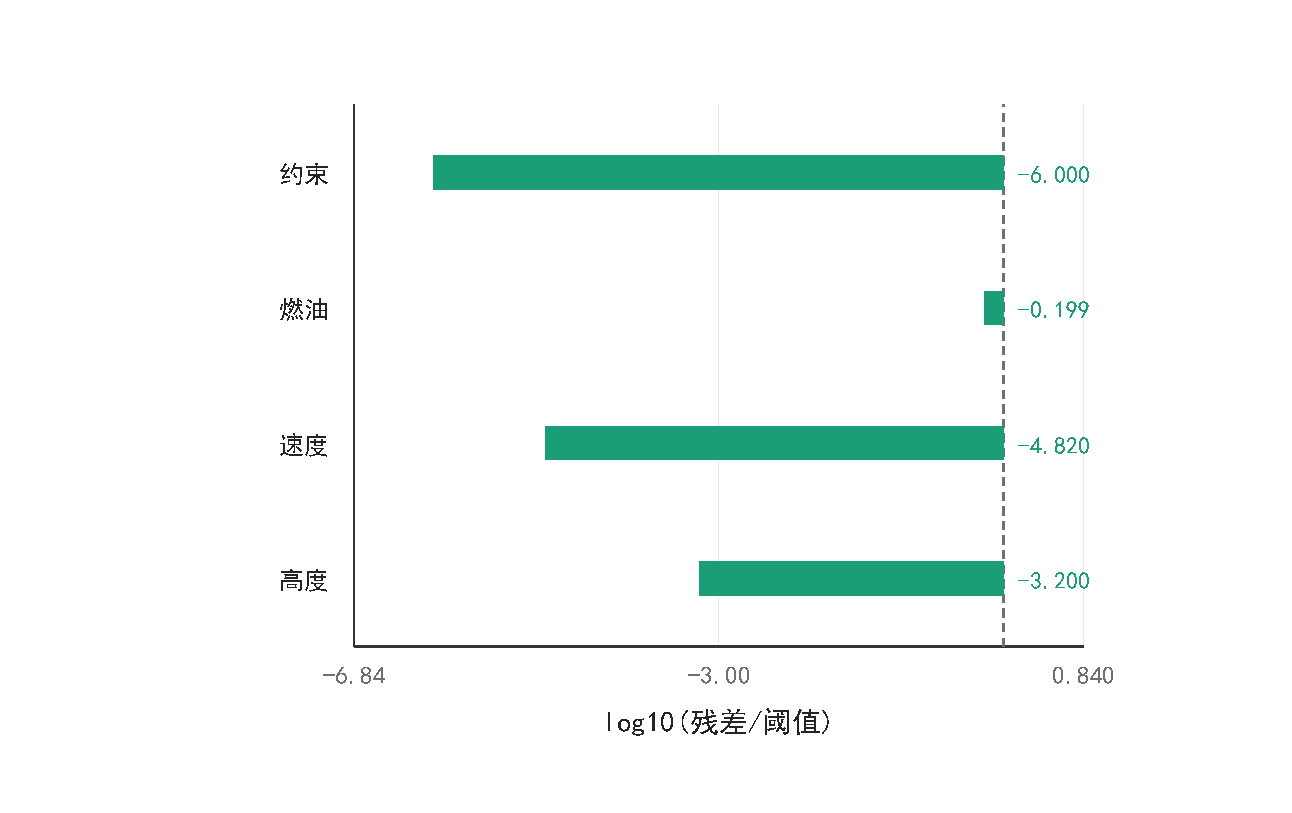
\includegraphics[width=0.82\textwidth]{fig_v2_q4_validation_card.pdf}
\caption{问题四有风局部优化的连续验证结果}
\label{fig:q4_validation_card}
\end{figure}

由图 \ref{fig:q4_validation_card} 可见，终端状态、燃油恒等式和路径约束均处于通过侧，说明标称有风局部优化轨迹具有连续动力学一致性。$\beta$ 五档扰动均通过终端状态和燃油恒等式验证，但非标称场景优化未达到最优终止条件，因此只支持局部可行敏感性。

\section{模型评价、改进与推广}

\subsection{模型的优点}
\begin{enumerate}[left=0pt]
    \item \textbf{动力学链条清晰，算法检验充分。} 采用小航迹角准稳态模型，清晰解耦状态变量关系；配合隐式多步积分与多重残差检验，有效排除了积分步长对仿真结果的偶然性干扰。\item \textbf{控制策略闭合，环境修正自洽。} 在缺乏推力包线时，引入参考升力系数闭合条件，确保等速与等马赫策略气动口径一致；大气修正满足静力平衡，避免了物理不一致性。\item \textbf{优化证据链分层，网格收敛可靠。} 采用直接配点法提供高质量可行初值，并通过最终网格稳定性和连续验证确认无风优化结果，确保轨迹结论的真实性与可靠性。
    \item \textbf{对比口径统一，结果解释客观。} 有风优化基于无风最优初值引入，采用固定航程与固定燃油双口径严密比较差异；结论完全基于当前模型数值证据，不预设主观倾向。
\end{enumerate}

\subsection{模型的缺点}
\begin{enumerate}[left=0pt]
    \item \textbf{动力学简化与工程约束不全。} 准稳态假设未考虑完整六自由度动力学，在大航迹角或强机动下适用性下降；且未引入跨音速波阻及空域控制等工程限制。
    \item \textbf{大气与气动控制律存在简化。} 混合大气模型在高度分层上精细度不足，后续需统一为分层标准大气；固定 $C_L$ 的闭合条件属于操作假设，无法代表真实的综合飞行控制律。
    \item \textbf{有风优化局限于局部解。} 有风算法采用低维控制结点参数化，在非标称场景下未完全达到最优终止条件，因此节油结论仅支持局部可行性，无法确证全局最优性。
\end{enumerate}

\subsection{模型的改进与推广}

\begin{enumerate}[left=0pt]
\item \textbf{统一大气模型。}采用分层标准大气模型替代指数密度近似，并保持温度、压力、密度和声速之间的静力一致性。
\item \textbf{补充飞机工程约束。}引入发动机推力包线、跨音速波阻项和空域高度限制，扩展模型在高马赫数巡航区域的应用范围。
\item \textbf{增强有风优化控制参数化。}在当前 5 个控制结点基础上增加结点数或采用稀疏 NLP 交叉验证，提高有风局部解的最优性保障。
\item \textbf{补充完整 Hamiltonian 诊断。}对有风最优轨迹构造协态和驻值条件，验证 PMP 必要条件的满足程度。
\end{enumerate}

% ============================================================
% 参考文献
% ============================================================
\newpage
\begin{thebibliography}{99}

\bibitem{raymer} Raymer D P. \emph{Aircraft Design: A Conceptual Approach}[M]. 6th ed. Reston, VA: AIAA, 2018.

\bibitem{anderson} Anderson J D. \emph{Fundamentals of Aerodynamics}[M]. 6th ed. New York: McGraw-Hill, 2017.

\bibitem{cook} Cook M V. \emph{Flight Dynamics Principles: A Linear Systems Approach to Aircraft Stability and Control}[M]. 3rd ed. Oxford: Butterworth-Heinemann, 2013.

\bibitem{icao_atmos} International Civil Aviation Organization. \emph{Manual of the ICAO Standard Atmosphere: extended to 80 kilometres (262500 feet)}[S]. 3rd ed. Montreal: ICAO, 1993.

\bibitem{pontryagin} Pontryagin L S, Boltyanskii V G, Gamkrelidze R V, Mishchenko E F. \emph{The Mathematical Theory of Optimal Processes}[M]. New York: Interscience Publishers, 1962.

\bibitem{hargraves} Hargraves C R, Paris S W. Direct trajectory optimization using nonlinear programming and collocation[J]. \emph{Journal of Guidance, Control, and Dynamics}, 1987, 10(4): 338--342.

\bibitem{betts} Betts J T. \emph{Practical Methods for Optimal Control and Estimation Using Nonlinear Programming}[M]. 2nd ed. Philadelphia: SIAM, 2010.

\bibitem{cots2022} Cots O, Gergaud J, Goubinat D, Wembe B. Singular versus boundary arcs for aircraft trajectory optimization in climbing phase[EB/OL]. arXiv:2212.06694, 2022. \url{https://arxiv.org/abs/2212.06694}.

\bibitem{park2015} Park S G, Clarke J-P. Vertical trajectory optimization to minimize environmental impact in the presence of wind[EB/OL]. arXiv:1508.01829, 2015. \url{https://arxiv.org/abs/1508.01829}.

\bibitem{jafarimoghaddam2023} Jafarimoghaddam A, Paw Y C, Bilimoria K D. Time-fuel-optimal navigation of a commercial aircraft considering gradual and discrete altitude change options[EB/OL]. arXiv:2305.13577, 2023. \url{https://arxiv.org/abs/2305.13577}.

\bibitem{scipy} Virtanen P, Gommers R, Oliphant T E, et al. SciPy 1.0: fundamental algorithms for scientific computing in Python[J]. \emph{Nature Methods}, 2020, 17(3): 261--272.

\bibitem{codex} Codex，GPT-5，OpenAI，2026-07-06 至 2026-07-08。
\bibitem{claude} Claude，xxxx，2026-07-06 至 2026-07-08。


\end{thebibliography}

% ============================================================
% 附录
% ============================================================
\appendix
\renewcommand{\thesection}{附录\Alph{section}}

\section*{附录A\quad AI 工具使用详情}
\addcontentsline{toc}{section}{附录A\quad AI 工具使用详情}

\begin{enumerate}[left=0pt]
\item 所用 AI 工具的名称及版本：Codex，GPT-5，OpenAI，2026-07-06 至 2026-07-08\cite{codex}；
\item 使用 AI 工具的具体目的与环节：辅助整理题面、检查模型文档证据链、撰写论文框架和四问正文草稿；在已有 Q1--Q4 结果基础上撰写摘要、问题一至问题四的模型建立与求解、灵敏度分析、模型检验和模型评价，组织正文插图和附录结构，并进行 \LaTeX{} 语法校验。核心算法、模型建立、结果判断和最终审核由参赛队人工完成。
\item 关键交互记录（重要提示词及 AI 的回复）：论文方面，提示词为"根据题目和仓库中已完成的 q1--q4 结果补充所有待填写部分，完成正文初稿，摘要关键词占一页，Q4 完成综合比较叙述"；AI 的回复为读取本地赛题、Q1--Q4 结果 CSV、证据链和写作规则后，撰写问题四有风最优控制模型、策略对比、航程估计、$\beta$ 灵敏度和扩展框架，并更新摘要 Q4 分段和收束段。代码方面，提示词为"检查仓库 Q4 结果并核对数据一致性"；AI 的回复为定位 Q4 pipeline 输出、验证结果表和灵敏度表，并用本地检查脚本核对 \LaTeX{} 引用、标签和环境平衡。
\item 对 AI 生成内容的采纳情况与人工修改情况：论文表述由 AI 基于题目和 Q1--Q4 证据链生成，数值结论均来自仓库已有计算结果（策略对比表、$\beta$ 灵敏度表、航程估计表等）；问题四有风优化结论限定为局部可行解，非标称 $\beta$ 场景未取得优化器成功终止标志已明确标注；所有模型口径、关键数值、图题、引用和最终表述由参赛队人工复核。
\end{enumerate}
\newpage
\section*{附录B\quad 主要程序代码}
\addcontentsline{toc}{section}{附录B\quad 主要程序代码}

\begin{table}[htpb]
\centering
\caption{主要程序文件说明}
\label{tab:program_files}
\begin{tabular}{p{9cm}p{6.5cm}}\toprule[1.5pt]
\textbf{程序文件} & \textbf{功能说明} \\
\midrule[1pt]
\multicolumn{2}{l}{\textbf{问题一}} \\
\path{q1/scripts/atmosphere.py} & 大气密度、声速与风场 \\
\path{q1/scripts/aircraft_model.py} & 气动参数与燃油模型 \\
\path{q1/scripts/strategy_constant_speed.py} & 等速策略高度--质量关系 \\
\path{q1/scripts/strategy_constant_mach.py} & 等马赫策略高度--质量关系 \\
\path{q1/scripts/simulate.py} & 两策略数值积分 \\
\path{q1/scripts/pipeline.py} & 求解入口与结果输出 \\
\multicolumn{2}{l}{\textbf{问题二}} \\
\path{q2/scripts/fuel_path_model.py} & 路径燃油积分与大气修正 \\
\path{q2/scripts/pipeline.py} & 主求解脚本 \\
\path{q2/scripts/validate.py} & 路径积分与敏感性验证 \\
\path{q2/scripts/visualize.py} & 图表生成脚本 \\
\multicolumn{2}{l}{\textbf{问题三}} \\
\path{q3/scripts/precheck.py} & 有风/无风可行性预检 \\
\path{q3/scripts/solve_feasibility_no_wind.py} & 无风 Gate 求解 \\
\path{q3/scripts/smooth_atmosphere.py} & 平滑温度与静力大气模型 \\
\path{q3/scripts/solve_feasibility_collocation_no_wind.py} & 配点与最终燃油优化 \\
\path{q3/scripts/validate.py} & 验证入口 \\
\path{q3/scripts/visualize.py} & 图表生成入口 \\
\multicolumn{2}{l}{\textbf{问题四}} \\
\path{q4/scripts/pipeline.py} & 有风 shooting 与灵敏度 \\
\path{q4/scripts/validate.py} & 终端状态与燃油验证 \\
\path{q4/scripts/visualize.py} & 论文级图表生成 \\
\bottomrule[1.5pt]
\end{tabular}
\end{table}

\subsection{主要源代码}

本节在最终提交前按需要补入主要源程序；当前版本先保留程序文件说明。

\end{document}
